
\documentclass[xcolor=table]{beamer}
\usepackage{appendixnumberbeamer}

\usepackage{subcaption}

% Change the margin
%\setbeamersize{text margin left = 2pt, text margin right = 2pt}

\setbeamertemplate{footline}[frame number]
\setbeamertemplate{headline}{}
% There are many different themes available for Beamer. A comprehensive
% list with examples is given here:
% http://deic.uab.es/~iblanes/beamer_gallery/index_by_theme.html
% You can uncomment the themes below if you would like to use a different
% one:
%\usetheme{AnnArbor}
%\usetheme{Antibes}
%\usetheme{Bergen}
%\usetheme{Berkeley}
%\usetheme{Berlin}
%\usetheme{Boadilla}
%\usetheme{boxes}
%\usetheme{CambridgeUS}
%\usetheme{Copenhagen}
%\usetheme{Darmstadt}
\usetheme{default}
%\usetheme{Frankfurt}
%\usetheme{Goettingen}
%\usetheme{Hannover}
%\usetheme{Ilmenau}
%\usetheme{JuanLesPins}
%\usetheme{Luebeck}
%\usetheme{Madrid}
%\usetheme{Malmoe}
%\usetheme{Marburg}
%\usetheme{Montpellier}
%\usetheme{PaloAlto}
%\usetheme{Pittsburgh}
%\usetheme{Rochester}
%\usetheme{Singapore}
%\usetheme{Szeged}
%\usetheme{Warsaw}
\makeatletter


\usepackage{fnpct}

\usepackage{subcaption}

\usepackage{newpxtext}


%fonts
\usefonttheme{professionalfonts}

%Other packages
\usepackage{bm}
\setbeamercovered{transparent}
\usepackage[section]{placeins}
\usepackage{epstopdf}
\usepackage[table]{xcolor}
\usepackage{graphicx} %Useful to resize large tables into the frame using \resizebox 
\usepackage{grffile} %Documentation: http://ctan.sharelatex.com/tex-archive/macros/latex/contrib/oberdiek/grffile.pdf
\usepackage{marvosym}
\usepackage[style=british]{csquotes}
\def\signed #1{{\leavevmode\unskip\nobreak\hfil\penalty50\hskip2em
		\hbox{}\nobreak\hfill #1
		\parfillskip=0pt \finalhyphendemerits=0 \endgraf}}

\newsavebox\mybox
\newenvironment{aquote}[1]
{\savebox\mybox{#1}\begin{quote}}
	{\vspace*{1mm}\signed{\usebox\mybox}\end{quote}}

\usepackage{verse}
\newcommand{\attrib}[1]{
	\nopagebreak{\raggedleft\footnotesize #1\par}}

%for checkmarks
\usepackage{tikz}

%For equations
\usepackage{amsmath, amssymb}
\usepackage{bbm}

%Tables
\usepackage{tabularx}
\usepackage{multirow}
\usepackage{multicol} 
\usepackage{booktabs}%\usepackage{booktabs, calc} %This is the package to use to have nice-looking tables. More documentation on the tables in LateX: https://www.tug.org/pracjourn/2007-1/mori/mori.pdf
\usepackage{threeparttable}  

\usepackage{lmodern}
\usepackage{booktabs}
\usepackage{pgfplots}

% Count slides
\setcounter{MaxMatrixCols}{10}

\graphicspath{{../figuras/}}
%\graphicspath{{../tablas/}}

% Commands -
\newcommand{\extractRGB}[1]{\extractcolorspecs{#1}{\model}{\dolphin} \convertcolorspec{\model}{\dolphin}{RGB}\printcol \printcol}
\setbeamertemplate{caption}{\raggedright\insertcaption\par} %to prevent beamer from putting "figure" in front of a caption
\setbeamertemplate{navigation symbols}{}

%Code to create sections with title pages in Beamer slides
\AtBeginSection[]{
	\begin{frame}[plain]
		\vfill
		\centering
		\begin{beamercolorbox}[sep=8pt,center,shadow=true,rounded=true]{title}
			\usebeamerfont{title}\insertsectionhead\par%
		\end{beamercolorbox}
		\vfill
	\end{frame}
}

\title{Sala Situacional COVID-19, Región Cusco\footnote{Análisis con información de la región hasta el 30 de octubre del 2021}}
\author{Fatima Concha} 
\institute{Dirección de Epidemiología e Investigación \\ \textbf{\color{mycolor3}DEIS, GERESA - Cusco}}
\date{Semana Epidemiológica 43, 2021 n}

\begin{document}
	%------------------------------------------------------------------------------------------------------------------------------------------------------------------------------------------------------------------------------------------
	% TITLE PAGE 
	%------------------------------------------------------------------------------------------------------------------------------------------------------------------------------------------------------------------------------------------
	\setbeamercovered{invisible}
	\begin{frame}[plain]
		\titlepage
	\end{frame}

	%------------------------------------------------------------------------------------------------------------------------------------------------------------------------------------------------------------------------------------------
	% INTRODUCTION 
	%------------------------------------------------------------------------------------------------------------------------------------------------------------------------------------------------------------------------------------------
	
	\setcounter{subsection}{1}
	\begin{frame}[label=indice]
		\frametitle{Índice}
		\vspace{-.5cm}
		\begin{itemize}
			\item Indicadores epidemiológicos.
			\begin{itemize}
				\item Nacional: Variantes, cobertura vacuna, mortalidad, RT, ocupación de camas UCI y no UCI a nivel regional. \hyperlink{epi_nacional}{\beamergotobutton{epi. nacional.}}
			\end{itemize} 
			\item Cobertura de Vacunación ({\color{mycolor5}Nuevo} \hyperlink{cobertura_vacuna}{\beamergotobutton{cobertura}}). 
			\item Indicadores de gestión hospitalaria.
			\item Resumen y recomendaciones. \hyperlink{resumen}{\beamergotobutton{resumen}} \hyperlink{recomendaciones}{\beamergotobutton{recomendaciones}}
			\item Links útiles. \hyperlink{links}{\beamergotobutton{links}} \hfill \hyperlink{vacunas_60}{\beamergotobutton{apendice}}
		\end{itemize}
	\end{frame}
	
	%------------------------------------------------------------------------------------------------------------------------------------------------------------------------------------------------------------------------------------------
	% SECCIÓN 1: Indicadores Epidemiológicos, Nivel Nacional
	%------------------------------------------------------------------------------------------------------------------------------------------------------------------------------------------------------------------------------------------
	\section{Indicadores Epidemiológicos, Nivel Nacional}

	\begin{frame}[label=epi_nacional]
	\frametitle{Tendencia de Variantes en Lima y la Sierra Selva Sur}
	\vspace{-.5cm}
	\begin{figure}
		\centering
		\begin{subfigure}[b]{0.45\textwidth}
			\centering
			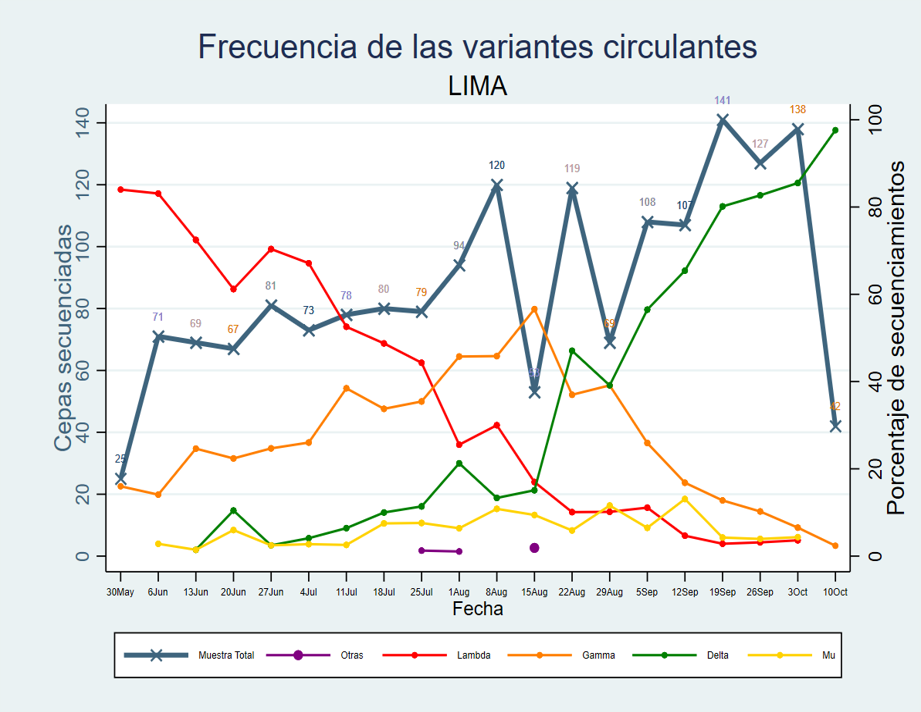
\includegraphics[width=\textwidth]{../sala_nacional/variantes_lima.png}
			\caption{Lima}
			%\label{fig:}
		\end{subfigure}
		\hfill
		\begin{subfigure}[b]{0.48\textwidth}
			\centering
			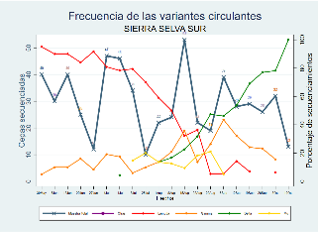
\includegraphics[width=\textwidth]{../sala_nacional/variantes_sierra_sur.png}
			\caption{Sierra Selva Sur}
			%\label{fig:70 a 79 años}
		\end{subfigure}
	\end{figure}
	{\tiny Fuente: Lescano, Orellana, Fano, Pino, y Flores. Situación Epidemiológica de la COVID-19 al 30 de octubre del 2021. \\
		Sierra Selva Sur: Apurimac, Ayacucho, Cusco, Madre de Dios, Puno. \\
		En Lima: Delta domina totalmente, ($ \sim100\% $), pocas muestras. Otras variantes casi desaparecen.\\
		Delta domina completamente en Lima y todas las macro-regiones. \\} 
	\vspace{0.01cm}
	$\rightarrow$ La variante delta (línea verde) se presenta con mayor frecuencia en la Sierra Selva Sur como en la capital. 
\end{frame}

%------------------------------------------------------------------------------------------------------------------------------------------------------------------------------------------------------------------------------------------
% SECCIÓN 2: Indicadores Epidemiológicos, Región Cusco
%------------------------------------------------------------------------------------------------------------------------------------------------------------------------------------------------------------------------------------------

	%-------------------------------------------------------------------------------------------------------------------------------------------------------------------------------------------------\textit{}-----------------------------------------
	% SECCIÓN 2: Indicadores de Gestión Hospitalaria
	%--------------------------------------------------------------------------------------------------------------------------------------------------------------------------------------------
	
	\begin{frame}[label=indicadores_provinciales]
		\frametitle{Tasa de Letalidad y Mortalidad, 2021}
		\vspace{-.5cm}
		
		% en el input de las tablas sólo debe comenzar y terminar con tabular, borrar el tabular de input de la tabla
		\begin{table}[]
			\resizebox{\textwidth}{!}{%
				\begin{tabular}{lccccc}
	\rowcolor[HTML]{DDEBF7} 
	\multicolumn{1}{c}{\cellcolor[HTML]{DDEBF7}\textbf{Provincias}} & \textbf{Población}   & \textbf{Total de  Pruebas} & \textbf{Defunciones} & \textbf{Tasa de letalidad} & \textbf{Tasa de mortalidad x   100,000 hab} \\
	\cellcolor[HTML]{FF5050}CANCHIS                                 & 105,049              & 4,325                      & 291                  & 6.7\%                      & 277.0                                       \\
	\cellcolor[HTML]{FF5050}CUSCO                                   & 463,656              & 41,999                     & 1,220                & 2.9\%                      & 263.1                                       \\
	\cellcolor[HTML]{FF5050}ANTA                                    & 57,731               & 2,358                      & 148                  & 6.3\%                      & 256.4                                       \\
	\cellcolor[HTML]{FF5050}QUISPICANCHI                            & 92,566               & 3,021                      & 218                  & 7.2\%                      & 235.5                                       \\
	\cellcolor[HTML]{F4B084}URUBAMBA                                & 66,439               & 3,153                      & 136                  & 4.3\%                      & 204.7                                       \\
	\cellcolor[HTML]{F4B084}CANAS                                   & 40,420               & 837                        & 67                   & 8.0\%                      & 165.8                                       \\
	\cellcolor[HTML]{F4B084}PARURO                                  & 31,264               & 567                        & 49                   & 8.6\%                      & 156.7                                       \\
	\cellcolor[HTML]{F4B084}LA CONVENCIÓN                           & 185,793              & 10,665                     & 290                  & 2.7\%                      & 156.1                                       \\
	\cellcolor[HTML]{FFE699}CHUMBIVILCAS                            & 84,925               & 1,976                      & 108                  & 5.5\%                      & 127.2                                       \\
	\cellcolor[HTML]{FFE699}PAUCARTAMBO                             & 52,989               & 949                        & 67                   & 7.1\%                      & 126.4                                       \\
	\cellcolor[HTML]{FFE699}ACOMAYO                                 & 28,477               & 706                        & 33                   & 4.7\%                      & 115.9                                       \\
	\cellcolor[HTML]{FFE699}CALCA                                   & 76,462               & 1,828                      & 74                   & 4.0\%                      & 96.8                                        \\
	\cellcolor[HTML]{FFE699}ESPINAR                                 & 71,304               & 2,075                      & 55                   & 2.7\%                      & 77.1                                        \\
	& \multicolumn{1}{l}{} & \multicolumn{1}{l}{}       & \multicolumn{1}{l}{} & \multicolumn{1}{l}{}       & \multicolumn{1}{l}{}                        \\
	\rowcolor[HTML]{DDEBF7} 
	\textbf{Total general}                                          & \textbf{1,357,075}   & \textbf{74,459}            & \textbf{2,756}       & \textbf{3.7\%}             & \textbf{203.1}                             
\end{tabular}
 
			}
		\end{table}
		{\tiny Fuente de datos: SINADEF. \hyperlink{indice}{\beamergotobutton{Índice}} \\} 
		
		Ver detalles de la tendencia (2020 y 2021) de estos indicadores para cada provincia haciendo clic en los siguientes enlaces:\\ \hyperlink{Acomayo}{\beamergotobutton{Acomayo}} \hyperlink{Anta}{\beamergotobutton{Anta}} \hyperlink{Calca}{\beamergotobutton{Calca}} \hyperlink{Canas}{\beamergotobutton{Canas}} \hyperlink{Chumbivilcas}{\beamergotobutton{Chimbivilcas}}
		\hyperlink{Canchis}{\beamergotobutton{Canchis}} \hyperlink{Cusco}{\beamergotobutton{Cusco}}
		\hyperlink{Espinar}{\beamergotobutton{Espinar}}
		\hyperlink{laconvencion}{\beamergotobutton{La Convencion}}
		\hyperlink{Paruro}{\beamergotobutton{Paruro}} \hyperlink{Paucartambo}{\beamergotobutton{Paucartambo}}
		\hyperlink{Quispicanchi}{\beamergotobutton{Quispicanchi}}
		\hyperlink{Urubamba}{\beamergotobutton{Urubamba}}
	\end{frame}

%-------------------------------------------------------------------------------------------------------------------------------------------------------------------------------------------------\textit{}-----------------------------------------
% SECCIÓN 4: Resúmen y Recomendaciones
%------------------------------------------------------------------------------------------------------------------------------------------------------------------------------------------------------------------------------------------
\section{Resumen }

\begin{frame}[label=resumen]
	\frametitle{Análisis Situacional por COVID-19: Resumen}
	\vspace{-.5cm}
	\begin{itemize}
		\item La Región de Cusco se ubica en el \textbf{\color{mycolor4}octavo lugar} de \textbf{\color{mycolor3}mortalidad} acumulada a nivel nacional, con una índice de propagación de $0.97 $.
		\item Continua la \textbf{\color{mycolor4}desaceleración sostenida} en el número de \textbf{\color{mycolor3}casos} y defunciones por COVID-19. 
		\item La \textbf{\color{mycolor3}tasa de positividad} para pruebas antigénicas se encuentra en mayor \textbf{\color{mycolor4}descenso} con un $4.8\%$, manteniéndose en este rango durante las últimas trece semanas. Mientras que, la \textbf{\color{mycolor3}tasa de positividad} para pruebas moleculares aumentó a un $16.9\%$ para la SE43.
		\end{itemize}
\end{frame}

\begin{frame}
	\frametitle{Análisis Situacional por COVID-19: Resumen}
	\vspace{-.5cm}
	\begin{itemize}
	\item La ocupación de camas \textbf{\color{mycolor3}UCI} aún es \textbf{\color{mycolor4} alta}, a pesar de haber disminuido a un $74\% $ y mantenerse como tal. 
	\item La ocupación de camas \textbf{\color{mycolor3}no UCI}, se ha mantenido en descenso con un $13\%$. \textbf{\color{mycolor4}} 
	\item La \textbf{\color{mycolor3}cobertura de vacunación regional} para COVID-19, muestra una \textbf{\color{mycolor4}cobertura por encima del 70\% para los grupos etarios mayores a 50 años}, con una brecha más amplia en los grupos etarios menores a 39 años.
	
	\end{itemize}
\end{frame}

\begin{frame}
	\frametitle{Análisis Situacional por COVID-19: Resumen}
	\vspace{-.5cm}
	\begin{itemize}
		\item Semáforo epidemiológico regional
		\begin{itemize}
			\item Tasa de crecimiento semanal de \textbf{\color{mycolor4}casos} en \textbf{\color{mycolor3}verde}.
			\item Tasa de crecimiento semanal de \textbf{\color{mycolor4}defunciones} en \textbf{\color{mycolor3}verde}.
			\item Tasa de \textbf{\color{mycolor4}positividad} de pruebas \textbf{\color{mycolor4}antigénicas} en verde y de prueba moleculares en ámbar.
			\item Disponibilidad de \textbf{\color{mycolor4}camas hospitalarias}: no UCI: en \textbf{\color{mycolor3}verde} el III y nivel II.
			\item Disponibilidad de camas hospitalarias: \textbf{\color{mycolor4}UCI} en \textbf{\color{mycolor3}rojo}.
		\end{itemize} 
		\item Semáforo epidemiológico a nivel provincial
		\begin{itemize}
			\item Todas las provincias presentan desaceleración de casos y defunciones para la SE 43. El exceso regional de mortalidad general es de -2.
	
		\end{itemize}
	\end{itemize}
\end{frame}

\begin{frame}[label=recomendaciones]
	\frametitle{Análisis Situacional por COVID-19: Recomendaciones}
	\vspace{-.5cm}
	\begin{itemize}
			\item Reforzar medidas de control por comandos C19 provinciales y distritales
			\item Campañas de comunicación, traducir mensajes claros, consistentes y constantes
			\item Énfasis en distanciamiento social, mascarilla, lavado de manos, aislamiento temprano si hay síntomas
			\item Asegurar aislamiento efectivo a personas con síntomas por 10 días y cuarentena de contactos cercanos por 14 días
			\item Aislamiento desde la llamada, no depender de la prueba
			\item Dar oxímetro, canasta de alimentos, monitoreo telefónico. 
			\item EPP bien usado – considerar que todos los pacientes son potenciales infectados
			\item Detectar y prevenir brotes nosocomiales
			
		\end{itemize} 

\end{frame}

\section{Links Útiles}

\begin{frame}[label=links]
	\frametitle{Links Útiles}
	\vspace{-.5cm}
	\begin{itemize}
		\item Encuentre {\color{mycolor4} información de la pandemia actualizada diaria a nivel regional, provincial, y distrital} en nuestro {\color{mycolor4}\textbf{Dashboard GERESA}} haciendo clic \href{https://geresacusco.shinyapps.io/DASHBOARD_COVID-19_CUSCO/}{\color{mycolor2}aquí}.
		\item Encuentre información actualizada de los {\color{mycolor4}Mapas de Calor COVID-19} en el haciendo clic \href{http://www.diresacusco.gob.pe/diresa/}{\color{mycolor2}aquí}.
		\item Encuentre información diaria del {\color{mycolor4} Resumen de la Sala Situacional COVID-19} de la Región haciendo clic \href{https://app.powerbi.com/view?r=eyJrIjoiZDdiMzA4YWMtZTZmNC00ZWE2LWFmMmYtODkwZmM1ODhiYTljIiwidCI6IjM2NGE0NmEwLTk0YzctNGZkNi1iYTNjLTlmMmQzMjA5YzFlZiJ9}{\color{mycolor2}aquí}.
		\item Encuentre información resumen cuatro semanas de la situación epidemiológica de COVID-19 en los {\color{mycolor4}Boletines COVID-19} haciendo clic \href{https://sites.google.com/view/geresacusco/boletines-epidemiologicos-covid-19}{\color{mycolor2}aquí}. \hyperlink{indice}{\beamergotobutton{Índice}}
	\end{itemize}

\end{frame}


%------------------------------------------------------------------------------------------------------------------------------------------------------------------------------------------------------------------------------------------
% APÉNDICE
%------------------------------------------------------------------------------------------------------------------------------------------------------------------------------------------------------------------------------------------

%\backupbegin

%\setbeamercovered{invisible}
%\begin{frame}[plain,noframenumbering]
%	\titlepage
%\end{frame}

\appendix
\section{Apéndice}

\subsection{Vacunación por Provincias y Grupo de Edad}

\begin{frame}[label=vacunas_70]
	\frametitle{Porcentaje de Cobertura de Vacunación de 70 a 79 años}
	\vspace{-.5cm}
	\begin{center}
		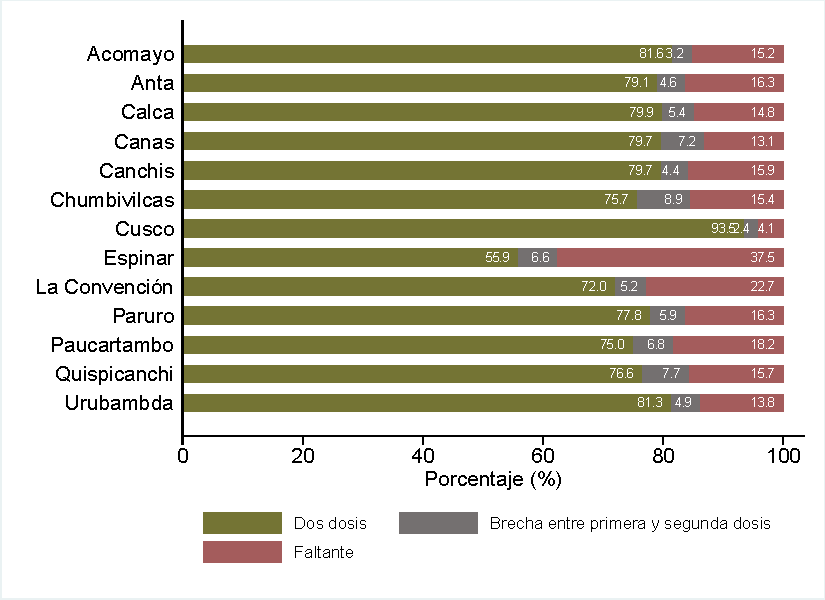
\includegraphics[width=0.8\linewidth, trim={.2cm .5cm .2cm .2cm},clip]{../figuras/vacunacion_provincial_edad_7.pdf}
	\end{center}
	{\tiny Fuente de datos: SICOVAC - HIS MINSA, Dirección de Estadística GERESA Cusco. \\}
\hyperlink{cobertura_vacuna_provincias}{\beamergotobutton{regresar}}
\end{frame}

\begin{frame}[label=vacunas_60]
	\frametitle{Porcentaje de Cobertura de Vacunación de 60 a 69 años, Provincias de Cusco}
	\vspace{-.5cm}
	\begin{center}
		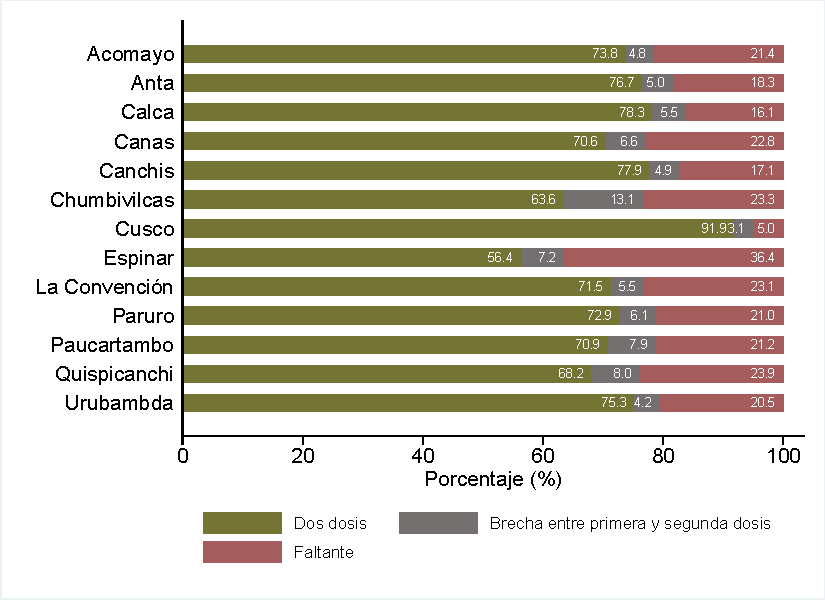
\includegraphics[width=0.8\linewidth, trim={.2cm .5cm .2cm .2cm},clip]{../figuras/vacunacion_provincial_edad_6.pdf}
	\end{center}
	{\tiny Fuente de datos: SICOVAC - HIS MINSA, Dirección de Estadística GERESA Cusco. \\}
	\hyperlink{cobertura_vacuna_provincias}{\beamergotobutton{regresar}}
\end{frame}

\begin{frame}[label=vacunas_50]
	\frametitle{Porcentaje de Cobertura de Vacunación de 50 a 59 años, Provincias de Cusco}
	\vspace{-.5cm}
	\begin{center}
		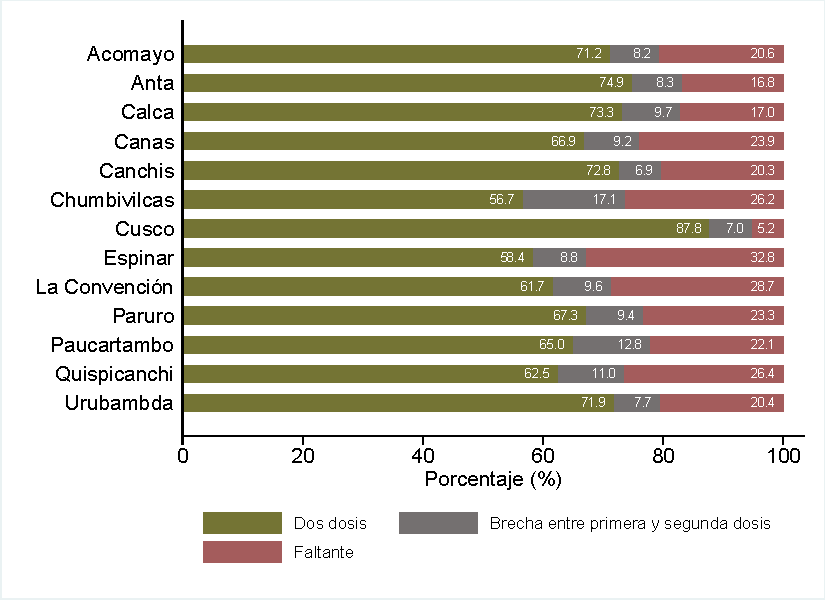
\includegraphics[width=0.8\linewidth, trim={.2cm .5cm .2cm .2cm},clip]{../figuras/vacunacion_provincial_edad_5.pdf}
	\end{center}
	{\tiny Fuente de datos: SICOVAC - HIS MINSA, Dirección de Estadística GERESA Cusco. \\}
\hyperlink{cobertura_vacuna_provincias}{\beamergotobutton{regresar}}
\end{frame}

\begin{frame}[label=vacunas_40]
	\frametitle{Porcentaje de Cobertura de Vacunación de 40 a 49 años, Provincias de Cusco}
	\vspace{-.5cm}
	\begin{center}
		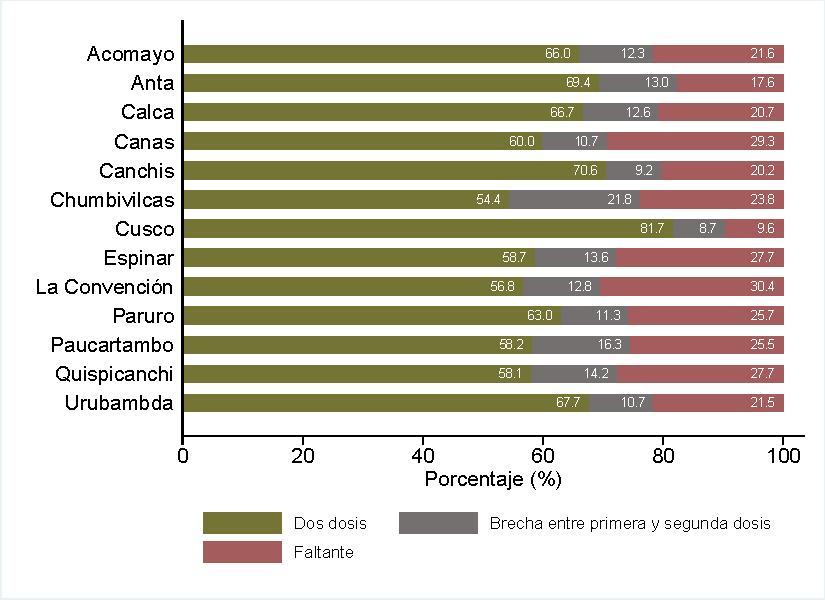
\includegraphics[width=0.8\linewidth, trim={.2cm .5cm .2cm .2cm},clip]{../figuras/vacunacion_provincial_edad_4.pdf}
	\end{center}
	{\tiny Fuente de datos: SICOVAC - HIS MINSA, Dirección de Estadística GERESA Cusco. \\}
\hyperlink{cobertura_vacuna_provincias}{\beamergotobutton{regresar}}
\end{frame}

\begin{frame}[label=vacunas_30]
	\frametitle{Porcentaje de Cobertura de Vacunación de 30 a 39 años, Provincias de Cusco}
	\vspace{-.5cm}
	\begin{center}
		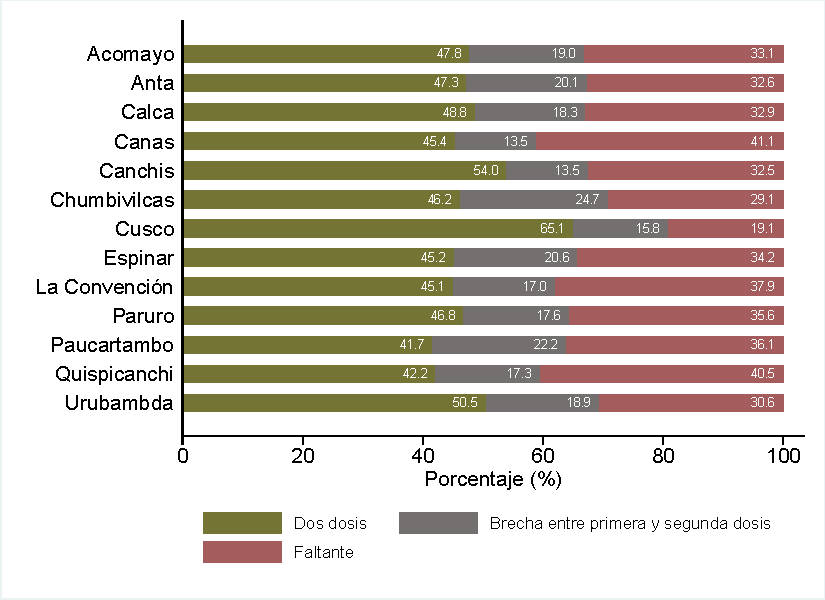
\includegraphics[width=0.8\linewidth, trim={.2cm .5cm .2cm .2cm},clip]{../figuras/vacunacion_provincial_edad_3.pdf}
	\end{center}
	{\tiny Fuente de datos: SICOVAC - HIS MINSA, Dirección de Estadística GERESA Cusco. \\}
\hyperlink{cobertura_vacuna_provincias}{\beamergotobutton{regresar}}
\end{frame}

\begin{frame}[label=vacunas_20]
	\frametitle{Porcentaje de Cobertura de Vacunación de 20 a 29 años, Provincias de Cusco}
	\vspace{-.5cm}
	\begin{center}
		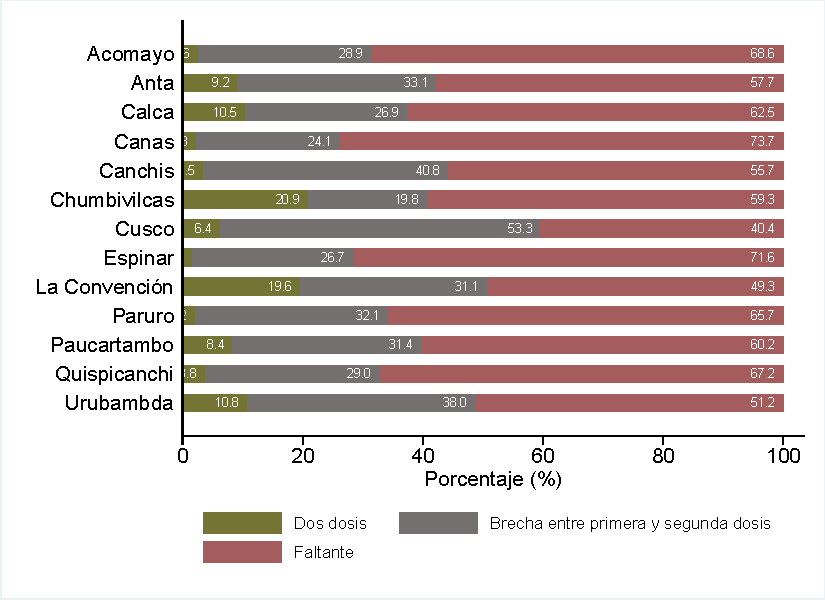
\includegraphics[width=0.8\linewidth, trim={.2cm .5cm .2cm .2cm},clip]{../figuras/vacunacion_provincial_edad_2.pdf}
	\end{center}
	{\tiny Fuente de datos: SICOVAC - HIS MINSA, Dirección de Estadística GERESA Cusco. \\}
\hyperlink{cobertura_vacuna_provincias}{\beamergotobutton{regresar}}
\end{frame}

\begin{frame}[label=vacunas_10]
	\frametitle{Porcentaje de Cobertura de Vacunación de 12 a 19 años, Provincias de Cusco}
	\vspace{-.5cm}
	\begin{center}
		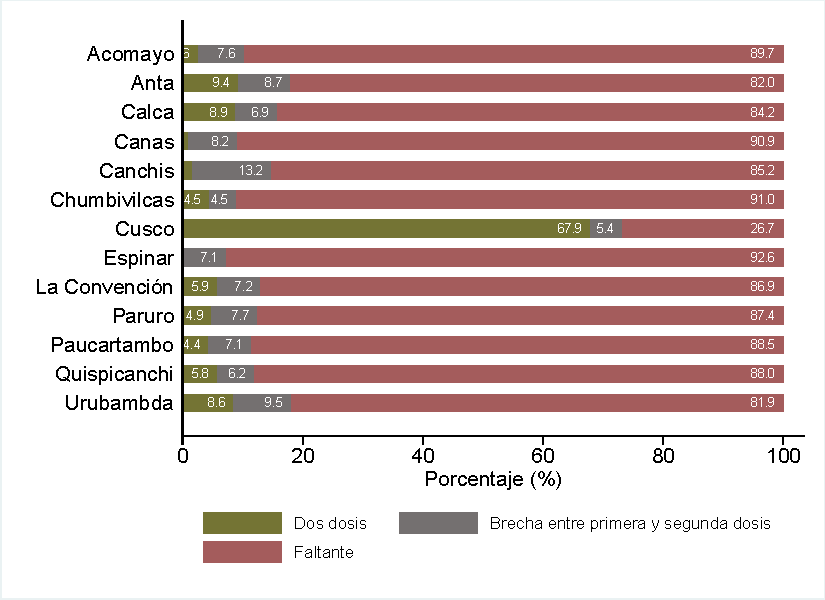
\includegraphics[width=0.8\linewidth, trim={.2cm .5cm .2cm .2cm},clip]{../figuras/vacunacion_provincial_edad_1.pdf}
	\end{center}
	{\tiny Fuente de datos: SICOVAC - HIS MINSA, Dirección de Estadística GERESA Cusco. \\}
\hyperlink{cobertura_vacuna_provincias}{\beamergotobutton{regresar}}
\end{frame}

\subsection{Acomayo}

\begin{frame}[label=Acomayo]
	\frametitle{Incidencia y Mortalidad, Provincia Acomayo}
	\vspace{-.5cm}
	\begin{center}
		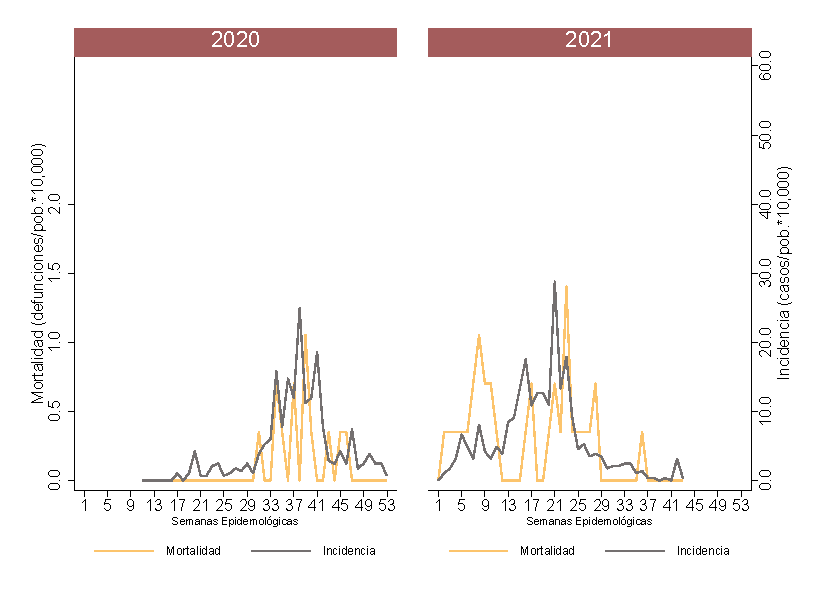
\includegraphics[width=0.8\linewidth, trim={0cm .5cm 0cm 0.2cm},clip]{../figuras/incidencia_mortalidad_20_21_1.pdf}
	\end{center}
	{\tiny Fuente de datos: SISCOVID, NOTICOVID, SINADEF.}
\end{frame}

\begin{frame}
	\frametitle{Tasa de Positividad, Provincia Acomayo}
	\vspace{-.5cm}
	\begin{center}
		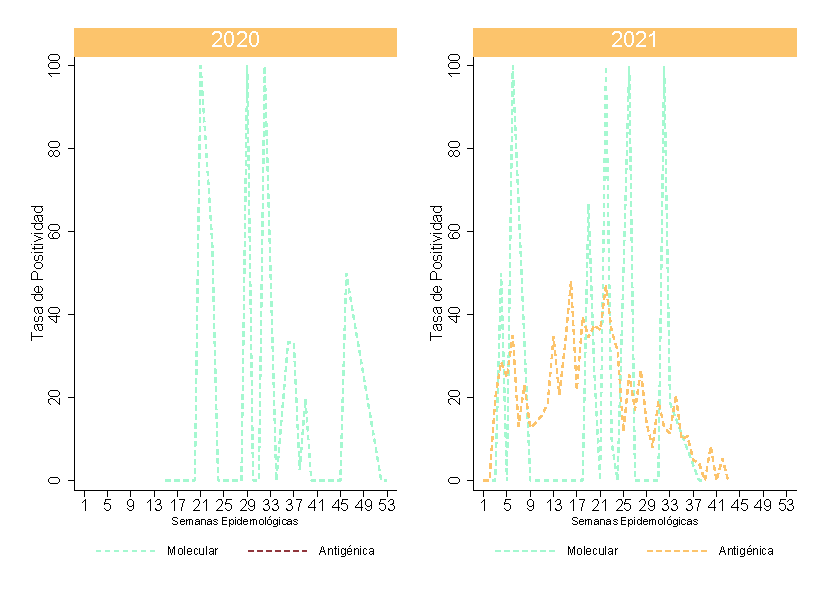
\includegraphics[width=0.8\linewidth, trim={0cm .5cm 0cm 0.2cm},clip]{../figuras/positividad_20_21_1.pdf}
	\end{center}
	{\tiny Fuente de datos: SISCOVID, NOTICOVID.}
\end{frame}

\begin{frame}
	\frametitle{Exceso de Defunciones por Todas las Causas, Provincia Acomayo}
	\vspace{-.5cm}
	\begin{center}
		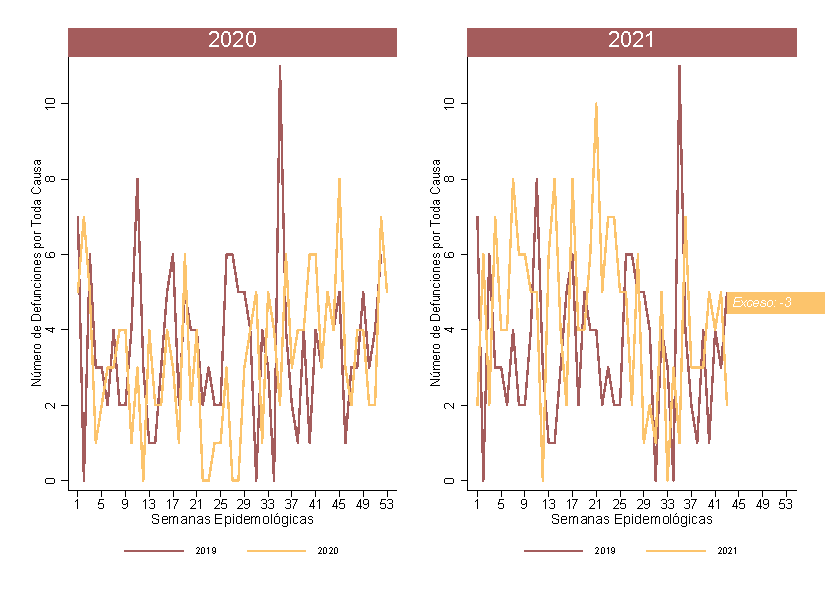
\includegraphics[width=0.8\linewidth, trim={0cm .5cm 0cm 0.2cm},clip]{../figuras/exceso_1.pdf}
	\end{center}
	{\tiny Fuente de datos: SINADEF.}
	
	\hyperlink{indicadores_provinciales}{\beamergotobutton{regresar}}
\end{frame}

\subsection{Anta}

\begin{frame}[label=Anta]
	\frametitle{Incidencia y Mortalidad, Provincia Anta}
	\vspace{-.5cm}
	\begin{center}
		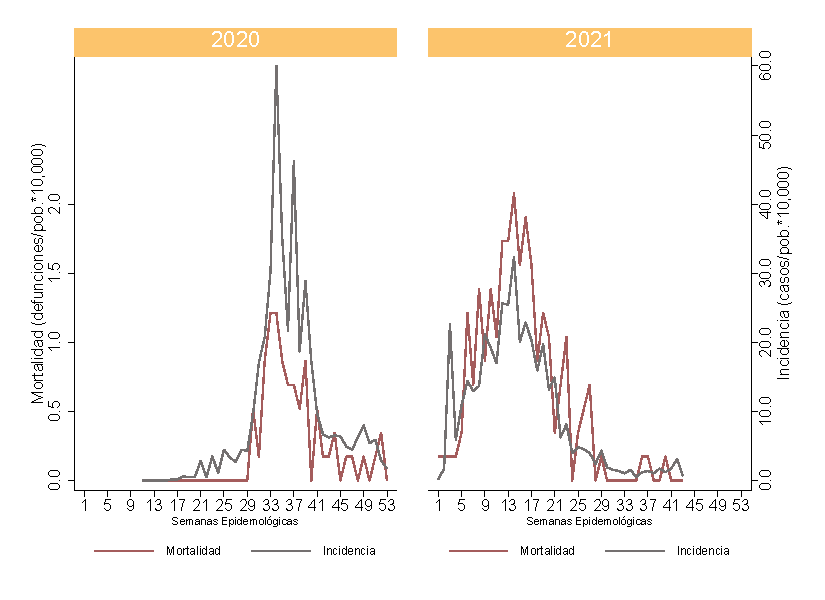
\includegraphics[width=0.8\linewidth, trim={0cm .5cm 0cm 0.2cm},clip]{../figuras/incidencia_mortalidad_20_21_2.pdf}
	\end{center}
	{\tiny Fuente de datos: SISCOVID, NOTICOVID, SINADEF.}
\end{frame}

\begin{frame}
	\frametitle{Tasa de Positividad, Provincia Anta}
	\vspace{-.5cm}
	\begin{center}
		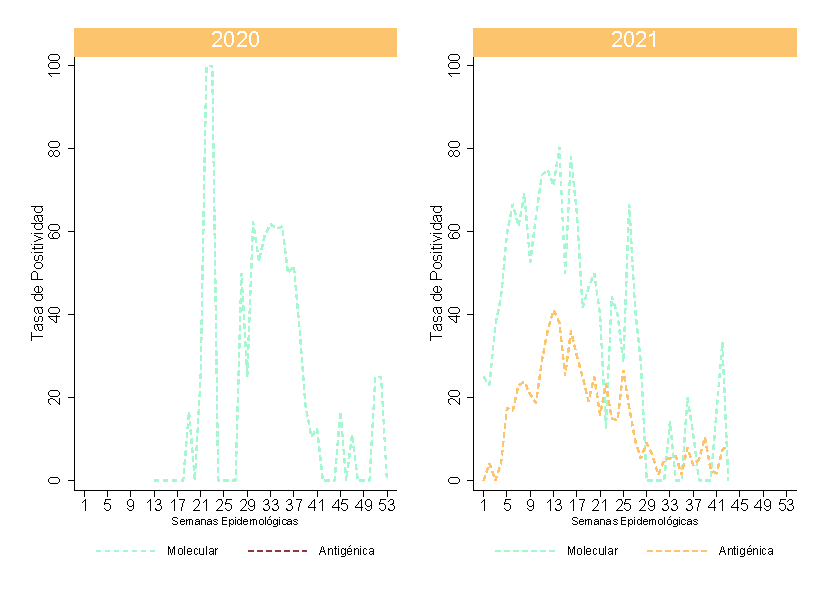
\includegraphics[width=0.8\linewidth, trim={0cm .5cm 0cm 0.2cm},clip]{../figuras/positividad_20_21_2.pdf}
	\end{center}
	{\tiny Fuente de datos: SISCOVID, NOTICOVID.}
\end{frame}

\begin{frame}
	\frametitle{Exceso de Defunciones por Todas las Causas, Provincia Anta}
	\vspace{-.5cm}
	\begin{center}
		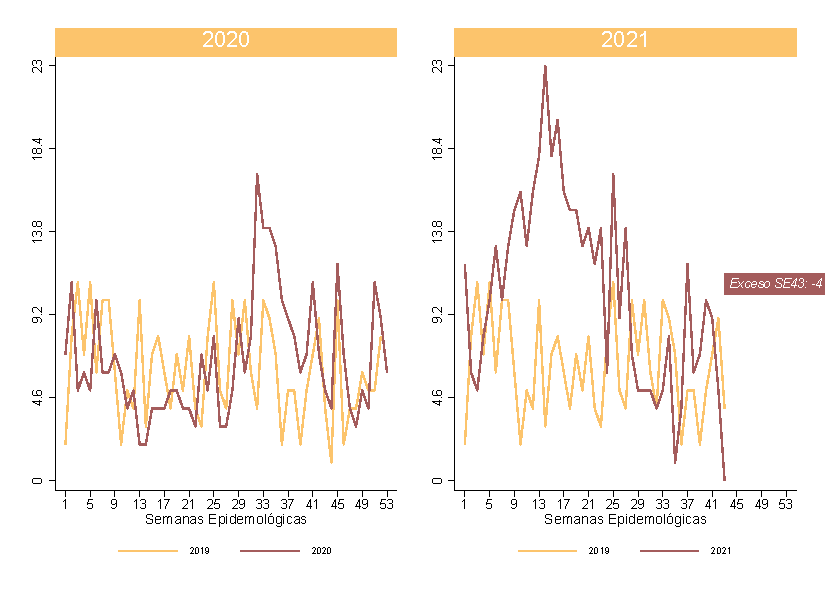
\includegraphics[width=0.8\linewidth, trim={0cm .5cm 0cm 0.2cm},clip]{../figuras/exceso_2.pdf}
	\end{center}
	{\tiny Fuente de datos: SINADEF.}
	
	\hyperlink{indicadores_provinciales}{\beamergotobutton{regresar}}
\end{frame}


\subsection{Calca}

\begin{frame}[label=Calca]
	\frametitle{Incidencia y Mortalidad, Provincia Calca}
	\vspace{-.5cm}
	\begin{center}
		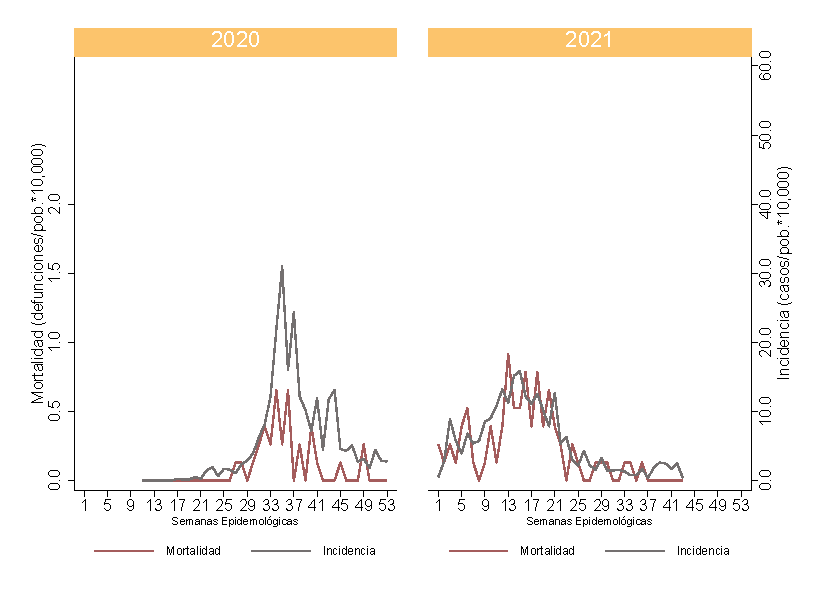
\includegraphics[width=0.8\linewidth, trim={0cm .5cm 0cm 0.2cm},clip]{../figuras/incidencia_mortalidad_20_21_3.pdf}
	\end{center}
	{\tiny Fuente de datos: SISCOVID, NOTICOVID, SINADEF.}
\end{frame}

\begin{frame}
	\frametitle{Tasa de Positividad, Provincia Calca}
	\vspace{-.5cm}
	\begin{center}
		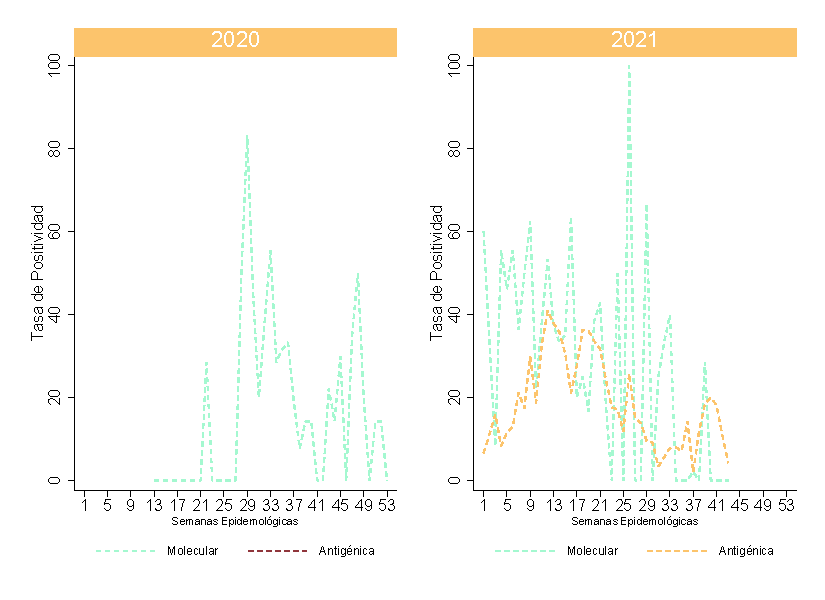
\includegraphics[width=0.8\linewidth, trim={0cm .5cm 0cm 0.2cm},clip]{../figuras/positividad_20_21_3.pdf}
	\end{center}
	{\tiny Fuente de datos: SISCOVID, NOTICOVID.}
\end{frame}

\begin{frame}
	\frametitle{Exceso de Defunciones por Todas las Causas, provincia Calca}
	\vspace{-.5cm}
	\begin{center}
		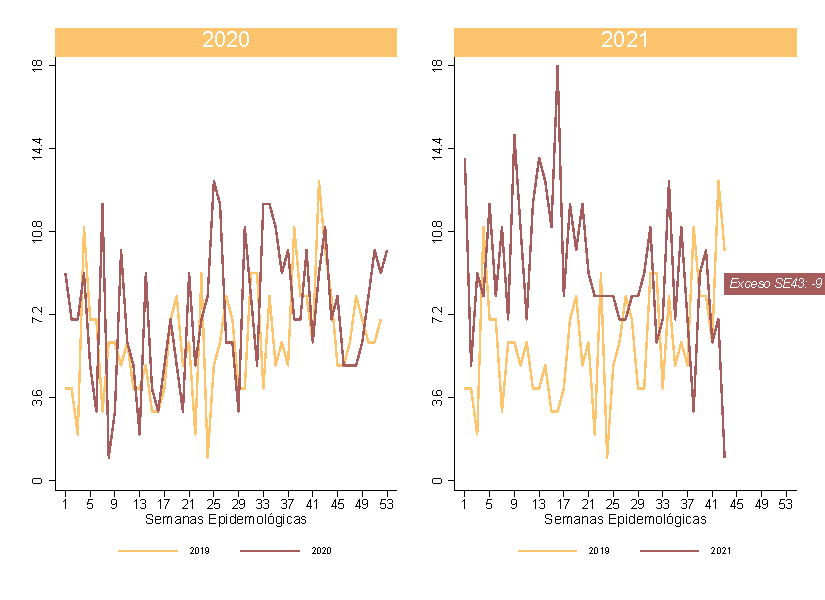
\includegraphics[width=0.8\linewidth, trim={0cm .5cm 0cm 0.2cm},clip]{../figuras/exceso_3.pdf}
	\end{center}
	{\tiny Fuente de datos: SINADEF.}
	
	\hyperlink{indicadores_provinciales}{\beamergotobutton{regresar}}
\end{frame}

\subsection{Canas}

\begin{frame}[label=Canas]
	\frametitle{Incidencia y Mortalidad, Provincia Canas}
	\vspace{-.5cm}
	\begin{center}
		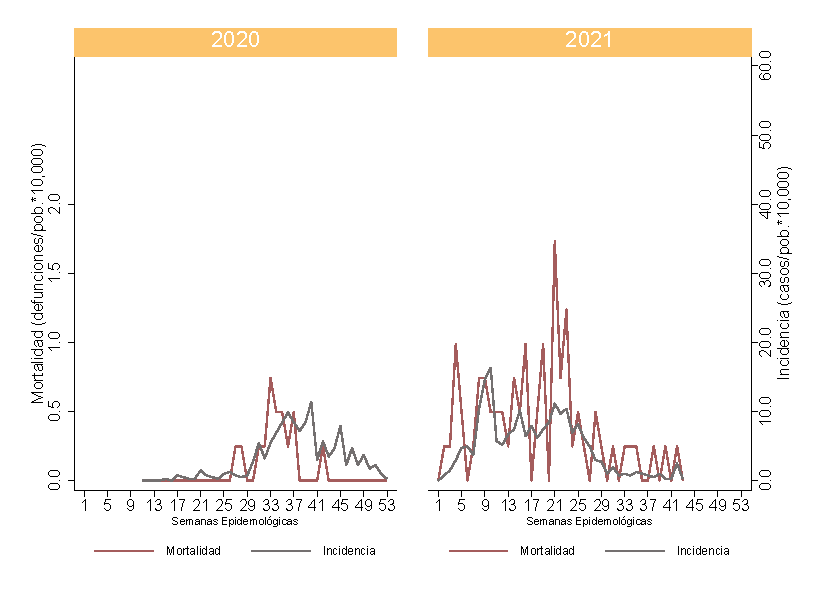
\includegraphics[width=0.8\linewidth, trim={0cm .5cm 0cm 0.2cm},clip]{../figuras/incidencia_mortalidad_20_21_4.pdf}
	\end{center}
	{\tiny Fuente de datos: SISCOVID, NOTICOVID, SINADEF}
\end{frame}

\begin{frame}
	\frametitle{Tasa de positividad, Provincia Canas}
	\vspace{-.5cm}
	\begin{center}
		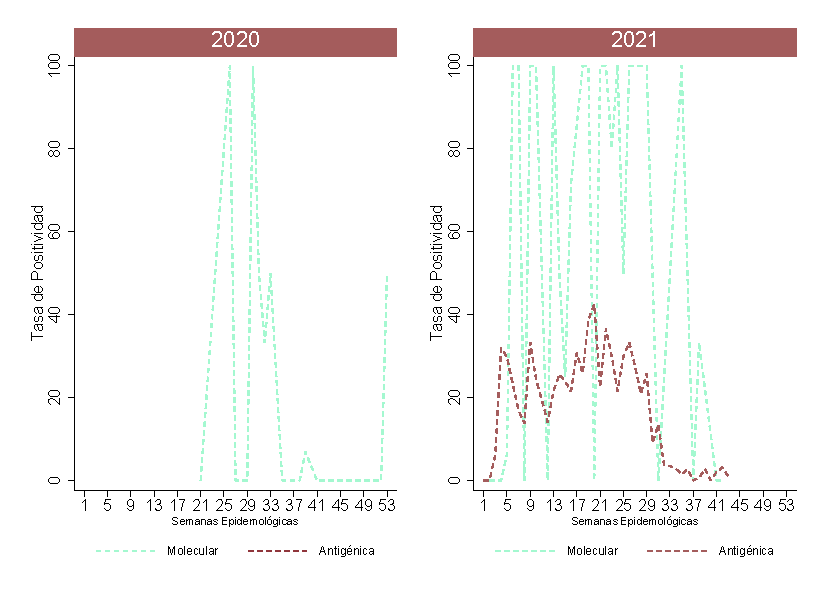
\includegraphics[width=0.8\linewidth, trim={0cm .5cm 0cm 0.2cm},clip]{../figuras/positividad_20_21_4.pdf}
	\end{center}
	{\tiny Fuente de datos: SISCOVID, NOTICOVID.}
\end{frame}

\begin{frame}
	\frametitle{Exceso de Defunciones por Todas las Causas, provincia Canas}
	\vspace{-.5cm}
	\begin{center}
		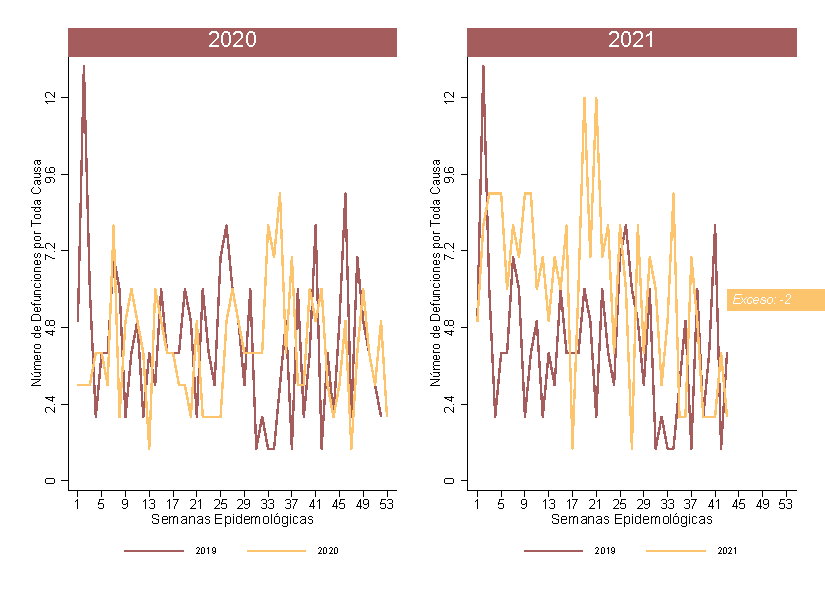
\includegraphics[width=0.8\linewidth, trim={0cm .5cm 0cm 0.2cm},clip]{../figuras/exceso_4.pdf}
	\end{center}
	{\tiny Fuente de datos: SINADEF.}
	
	\hyperlink{indicadores_provinciales}{\beamergotobutton{regresar}}
\end{frame}

\subsection{Canchis}

\begin{frame}[label=Canchis]
	\frametitle{Incidencia y Mortalidad, Provincia Canchis}
	\vspace{-.5cm}
	\begin{center}
		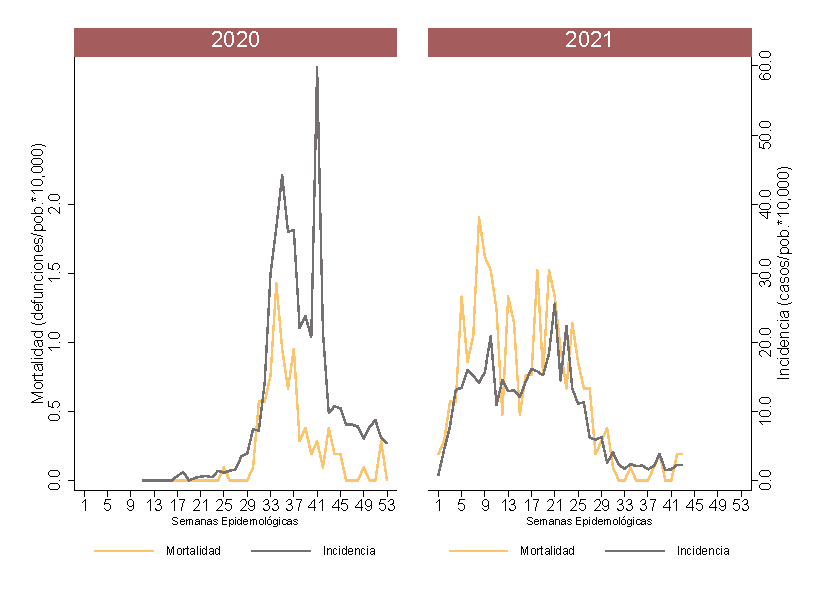
\includegraphics[width=0.8\linewidth, trim={0cm .5cm 0cm 0.2cm},clip]{../figuras/incidencia_mortalidad_20_21_5.pdf}
	\end{center}
	{\tiny Fuente de datos: SISCOVID, NOTICOVID, SINADEF}
\end{frame}

\begin{frame}
	\frametitle{Tasa de Positividad, Provincia Canchis}
	\vspace{-.5cm}
	\begin{center}
		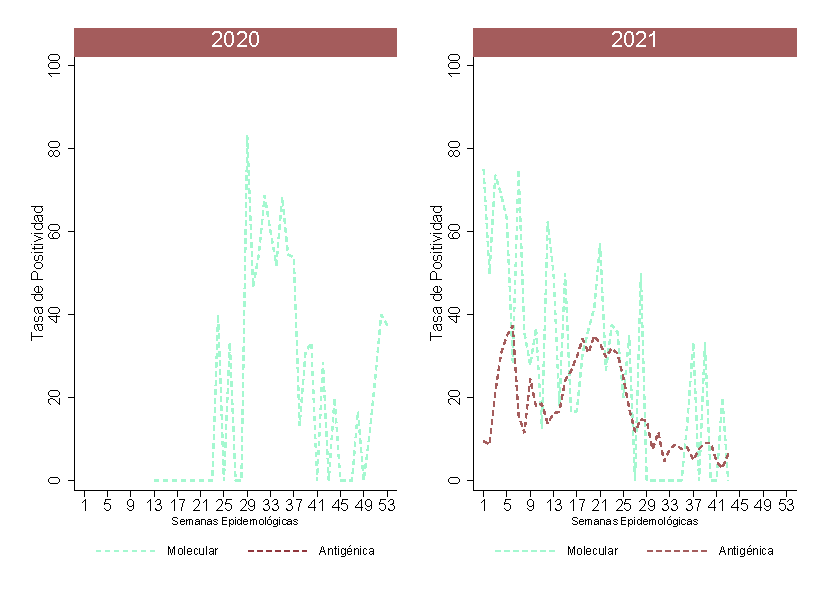
\includegraphics[width=0.8\linewidth, trim={0cm .5cm 0cm 0.2cm},clip]{../figuras/positividad_20_21_5.pdf}
	\end{center}
	{\tiny Fuente de datos: SISCOVID, NOTICOVID.}
\end{frame}

\begin{frame}
	\frametitle{Exceso de Defunciones por Todas las Causas, Provincia Canchis}
	\vspace{-.5cm}
	\begin{center}
		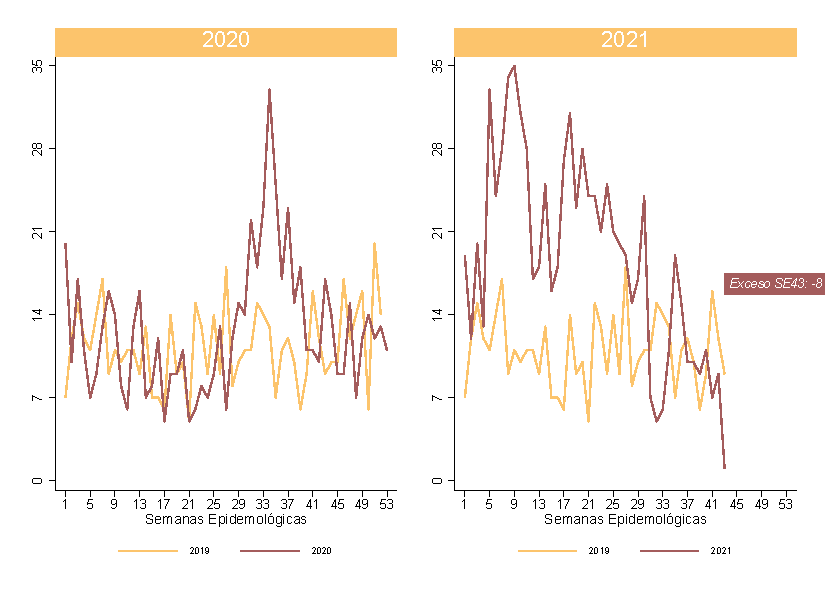
\includegraphics[width=0.8\linewidth, trim={0cm .5cm 0cm 0.2cm},clip]{../figuras/exceso_5.pdf}
	\end{center}
	{\tiny Fuente de datos: SINADEF.}
	
	\hyperlink{indicadores_provinciales}{\beamergotobutton{regresar}}
\end{frame}

\subsection{Chumbivilcas}

\begin{frame}[label=Chumbivilcas]
	\frametitle{Incidencia y Mortalidad, Provincia Chumbivilcas}
	\vspace{-.5cm}
	\begin{center}
		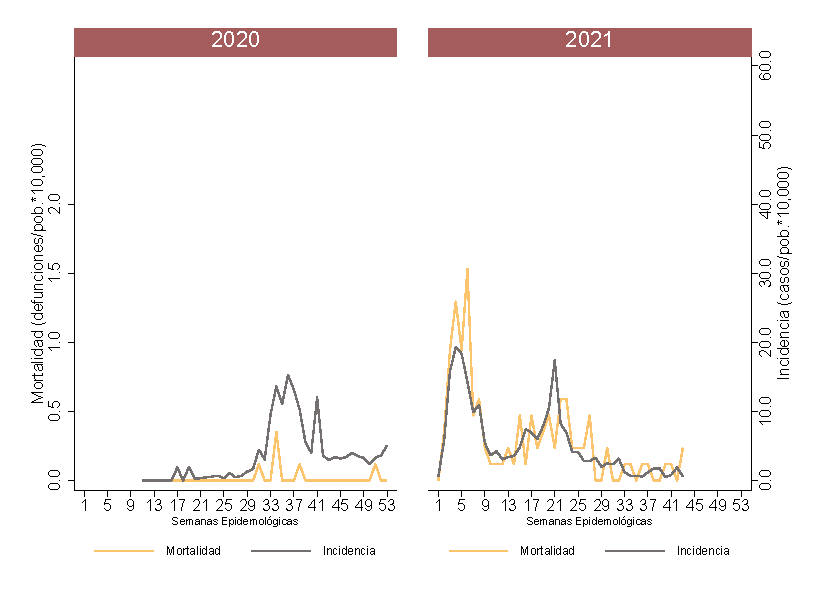
\includegraphics[width=0.8\linewidth, trim={0cm .5cm 0cm 0.2cm},clip]{../figuras/incidencia_mortalidad_20_21_6.pdf}
	\end{center}
	{\tiny Fuente de datos: SISCOVID, NOTICOVID, SINADEF}
\end{frame}

\begin{frame}
	\frametitle{Tasa de Positividad, Provincia Chumbivilcas}
	\vspace{-.5cm}
	\begin{center}
		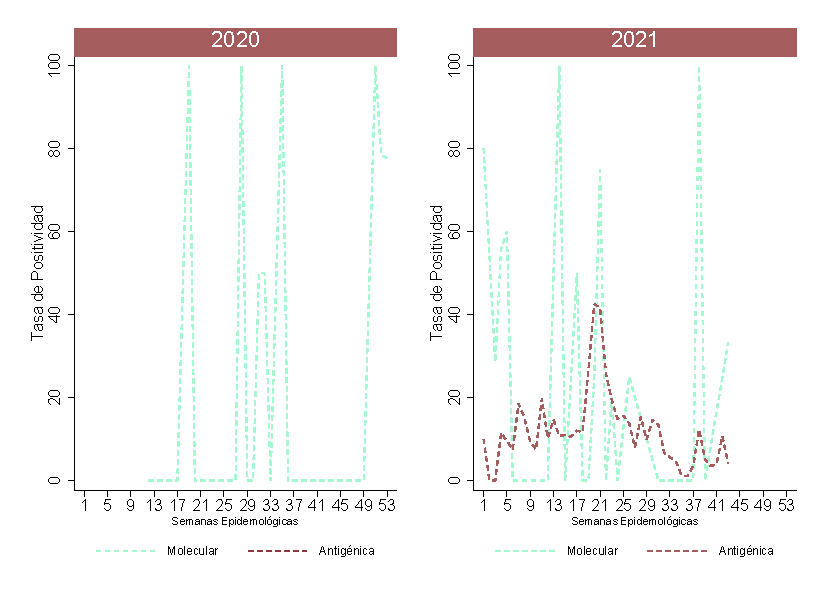
\includegraphics[width=0.8\linewidth, trim={0cm .5cm 0cm 0.2cm},clip]{../figuras/positividad_20_21_6.pdf}
	\end{center}
	{\tiny Fuente de datos: SISCOVID, NOTICOVID.}
\end{frame}

\begin{frame}
	\frametitle{Exceso de Defunciones por Todas las Causas, Provincia Chumbivilcas}
	\vspace{-.5cm}
	\begin{center}
		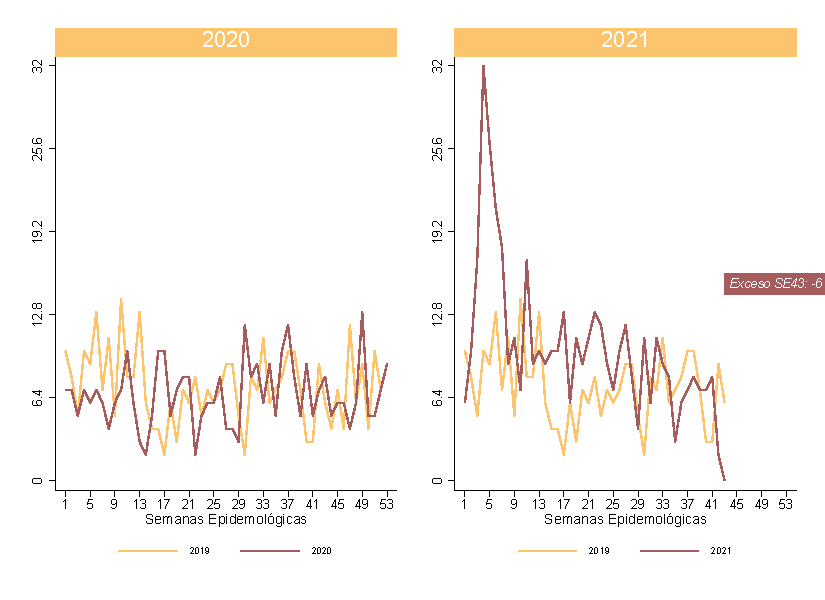
\includegraphics[width=0.8\linewidth, trim={0cm .5cm 0cm 0.2cm},clip]{../figuras/exceso_6.pdf}
	\end{center}
	{\tiny Fuente de datos: SINADEF.}
	
	\hyperlink{indicadores_provinciales}{\beamergotobutton{regresar}}
\end{frame}

\subsection{Cusco}

\begin{frame}[label=Cusco]
	\frametitle{Incidencia y Mortalidad, Provincia Cusco}
	\vspace{-.5cm}
	\begin{center}
		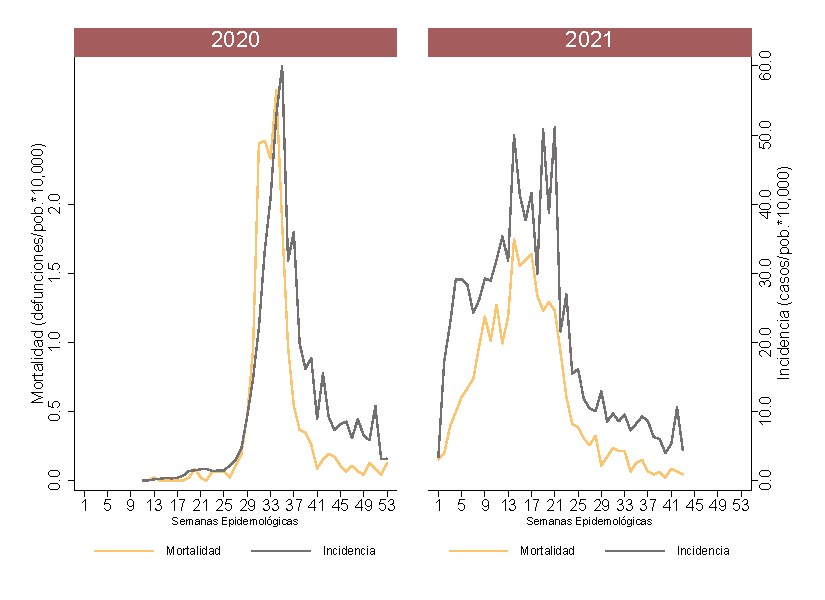
\includegraphics[width=0.8\linewidth, trim={0cm .5cm 0cm 0.2cm},clip]{../figuras/incidencia_mortalidad_20_21_7.pdf}
	\end{center}
	{\tiny Fuente de datos: SISCOVID, NOTICOVID, SINADEF.}
\end{frame}

\begin{frame}
	\frametitle{Tasa de Positividad, Provincia Cusco}
	\vspace{-.5cm}
	\begin{center}
		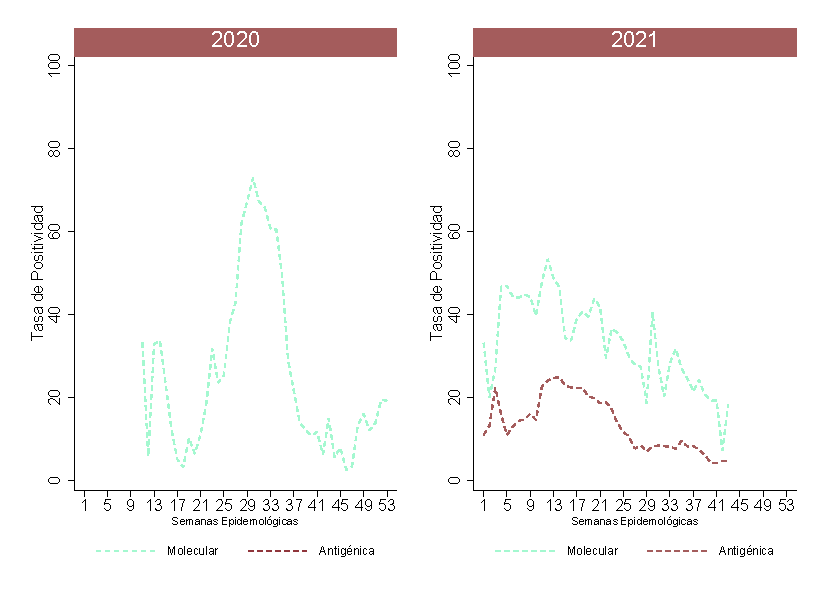
\includegraphics[width=0.8\linewidth, trim={0cm .5cm 0cm 0.2cm},clip]{../figuras/positividad_20_21_7.pdf}
	\end{center}
	{\tiny Fuente de datos: SISCOVID, NOTICOVID.}
\end{frame}

\begin{frame}
	\frametitle{Exceso de Defunciones por Todas las Causas, Provincia Cusco}
	\vspace{-.5cm}
	\begin{center}
		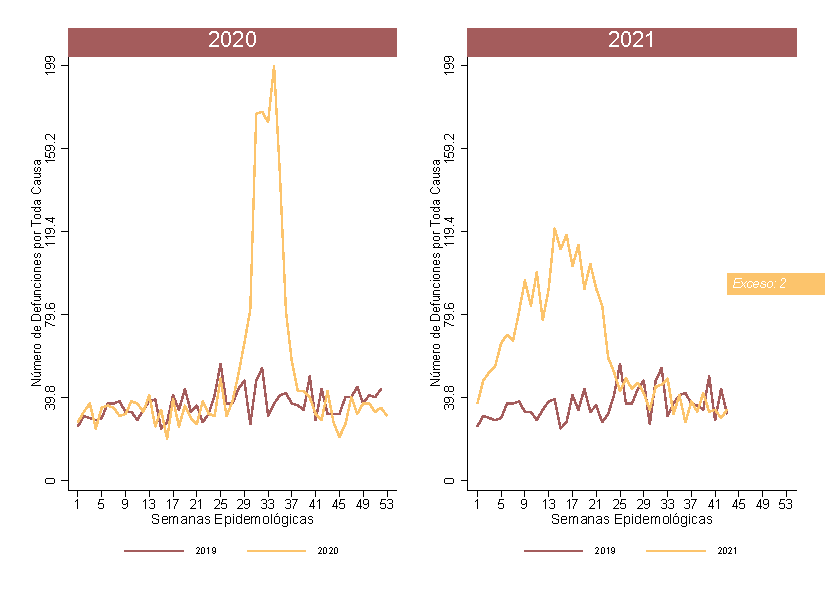
\includegraphics[width=0.8\linewidth, trim={0cm .5cm 0cm 0.2cm},clip]{../figuras/exceso_7.pdf}
	\end{center}
	{\tiny Fuente de datos: SINADEF.}
	
	\hyperlink{indicadores_provinciales}{\beamergotobutton{regresar}}
\end{frame}

\subsection{Espinar}

\begin{frame}[label=Espinar]
	\frametitle{Incidencia y Mortalidad, Provincia Espinar}
	\vspace{-.5cm}
	\begin{center}
		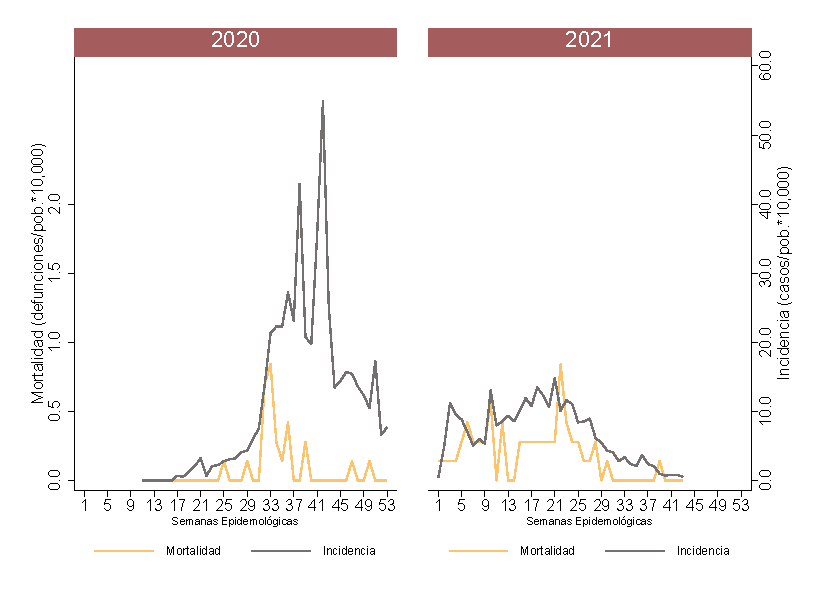
\includegraphics[width=0.8\linewidth, trim={0cm .5cm 0cm 0.2cm},clip]{../figuras/incidencia_mortalidad_20_21_8.pdf}
	\end{center}
	{\tiny Fuente de datos: SISCOVID, NOTICOVID, SINADEF.}
\end{frame}

\begin{frame}
	\frametitle{Tasa de Positividad, Provincia Espinar}
	\vspace{-.5cm}
	\begin{center}
		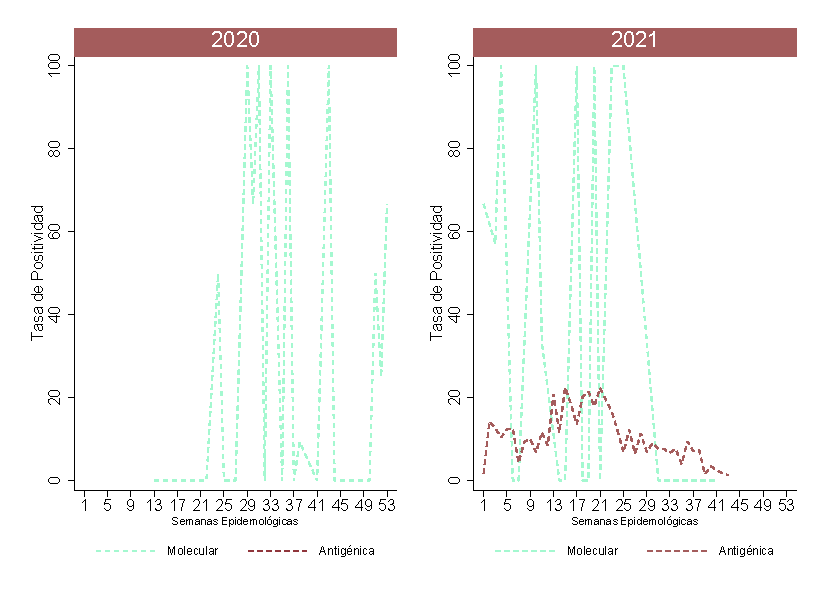
\includegraphics[width=0.8\linewidth, trim={0cm .5cm 0cm 0.2cm},clip]{../figuras/positividad_20_21_8.pdf}
	\end{center}
	{\tiny Fuente de datos: SISCOVID, NOTICOVID.}
\end{frame}

\begin{frame}
	\frametitle{Exceso de Defunciones por Todas las Causas, Provincia Espinar}
	\vspace{-.5cm}
	\begin{center}
		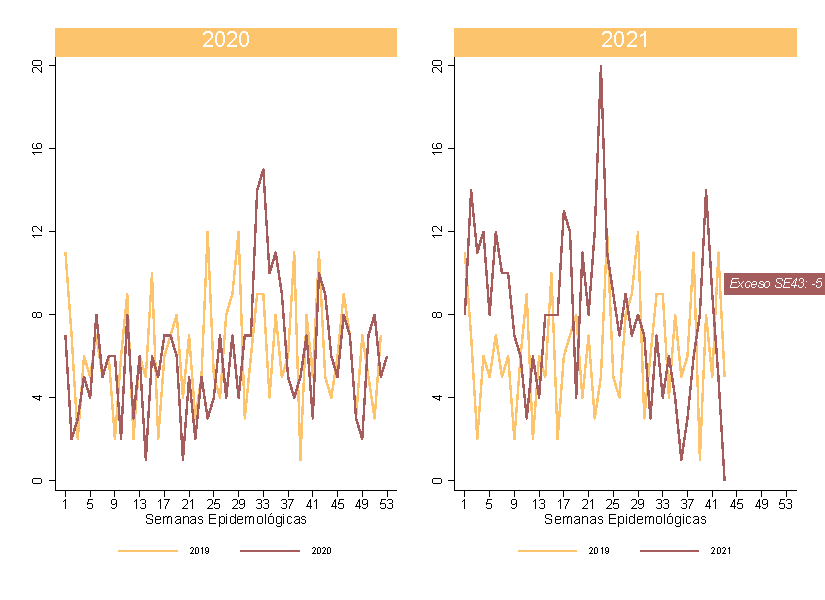
\includegraphics[width=0.8\linewidth, trim={0cm .5cm 0cm 0.2cm},clip]{../figuras/exceso_8.pdf}
	\end{center}
	{\tiny Fuente de datos: SINADEF.}
	
	\hyperlink{indicadores_provinciales}{\beamergotobutton{regresar}}
\end{frame}


\subsection{La Convención}

\begin{frame}[label=laconvencion]
	\frametitle{Incidencia y Mortalidad, Provincia La Convención}
	\vspace{-.5cm}
	\begin{center}
		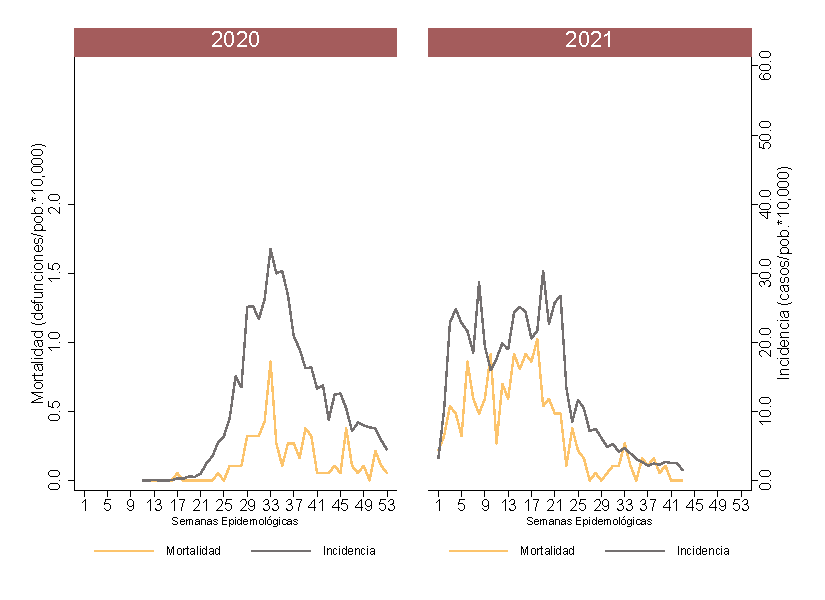
\includegraphics[width=0.8\linewidth, trim={0cm .5cm 0cm 0.2cm},clip]{../figuras/incidencia_mortalidad_20_21_9.pdf}
	\end{center}
	{\tiny Fuente de datos: SISCOVID, NOTICOVID, SINADEF.}
\end{frame}


\begin{frame}
	\frametitle{Exceso de Defunciones por Todas las Causas, Provincia Paruro}
	\vspace{-.5cm}
	\begin{center}
		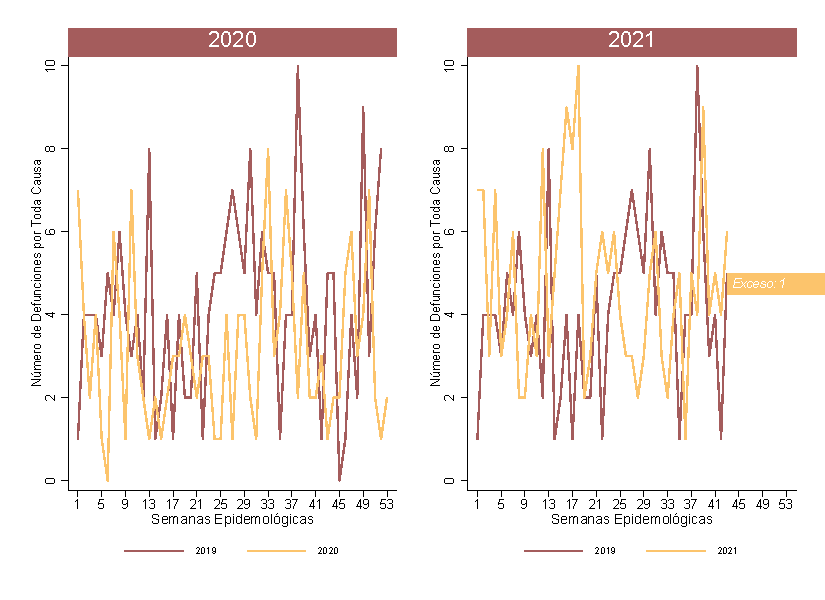
\includegraphics[width=0.8\linewidth, trim={0cm .5cm 0cm 0.2cm},clip]{../figuras/exceso_10.pdf}
	\end{center}
	{\tiny Fuente de datos: SINADEF.}
	
	\hyperlink{indicadores_provinciales}{\beamergotobutton{regresar}}
\end{frame}

\subsection{Paucartambo}

\begin{frame}[label=Paucartambo]
	\frametitle{Incidencia y Mortalidad, Provincia Paucartambo}
	\vspace{-.5cm}
	\begin{center}
		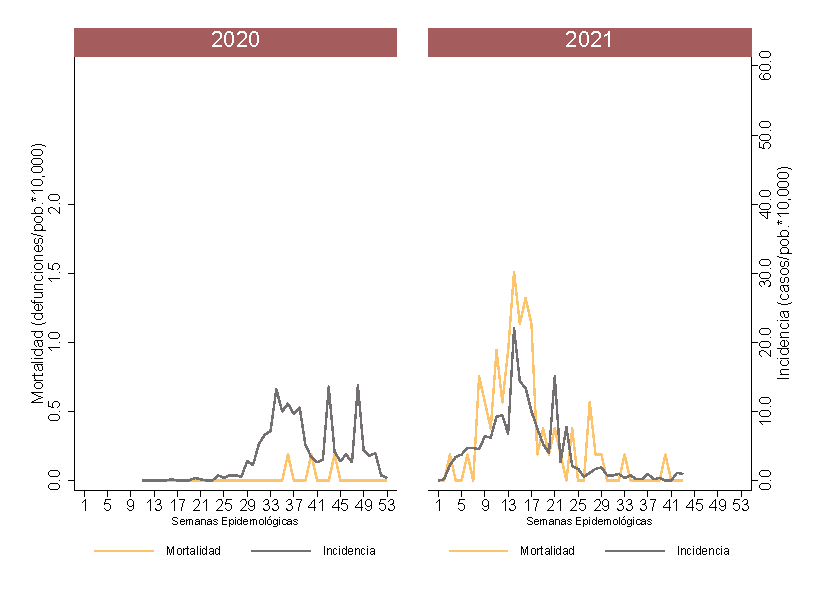
\includegraphics[width=0.8\linewidth, trim={0cm .5cm 0cm 0.2cm},clip]{../figuras/incidencia_mortalidad_20_21_11.pdf}
	\end{center}
	{\tiny Fuente de datos: SISCOVID, NOTICOVID, SINADEF.}
\end{frame}

\begin{frame}
	\frametitle{Tasa de Positividad, Provincia Paucartambo}
	\vspace{-.5cm}
	\begin{center}
		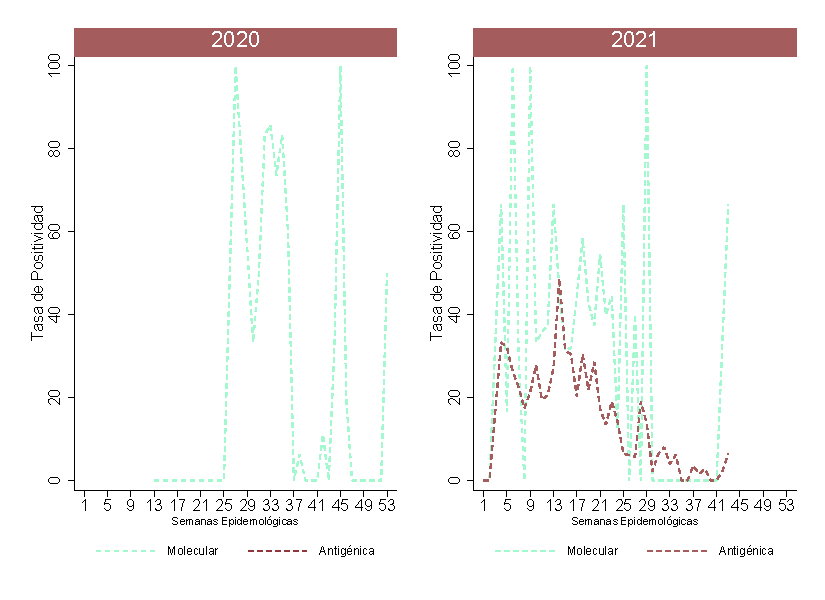
\includegraphics[width=0.8\linewidth, trim={0cm .5cm 0cm 0.2cm},clip]{../figuras/positividad_20_21_11.pdf}
	\end{center}
	{\tiny Fuente de datos: SISCOVID, NOTICOVID.}
\end{frame}

\begin{frame}
	\frametitle{Exceso de Defunciones por Todas las causas, provincia Paucartambo}
	\vspace{-.5cm}
	\begin{center}
		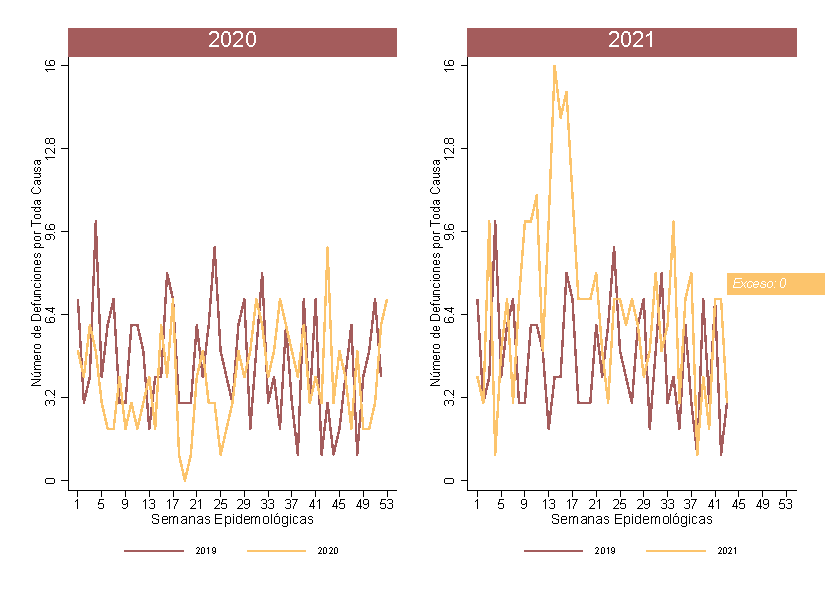
\includegraphics[width=0.8\linewidth, trim={0cm .5cm 0cm 0.2cm},clip]{../figuras/exceso_11.pdf}
	\end{center}
	{\tiny Fuente de datos: SINADEF.}
	
	\hyperlink{indicadores_provinciales}{\beamergotobutton{regresar}}
\end{frame}


\subsection{Quispicanchi}

\begin{frame}[label=Quispicanchi]
	\frametitle{Incidencia y Mortalidad, Provincia Quispicanchi}
	\vspace{-.5cm}
	\begin{center}
		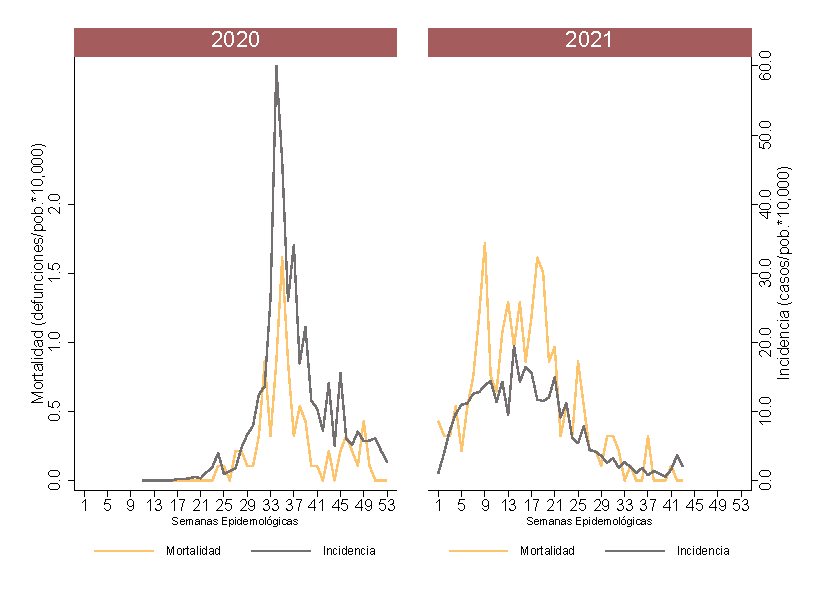
\includegraphics[width=0.8\linewidth, trim={0cm .5cm 0cm 0.2cm},clip]{../figuras/incidencia_mortalidad_20_21_12.pdf}
	\end{center}
	{\tiny Fuente de datos: SISCOVID, NOTICOVID, SINADEF.}
\end{frame}

\begin{frame}
	\frametitle{Tasa de Positividad, Provincia Quispicanchi}
	\vspace{-.5cm}
	\begin{center}
		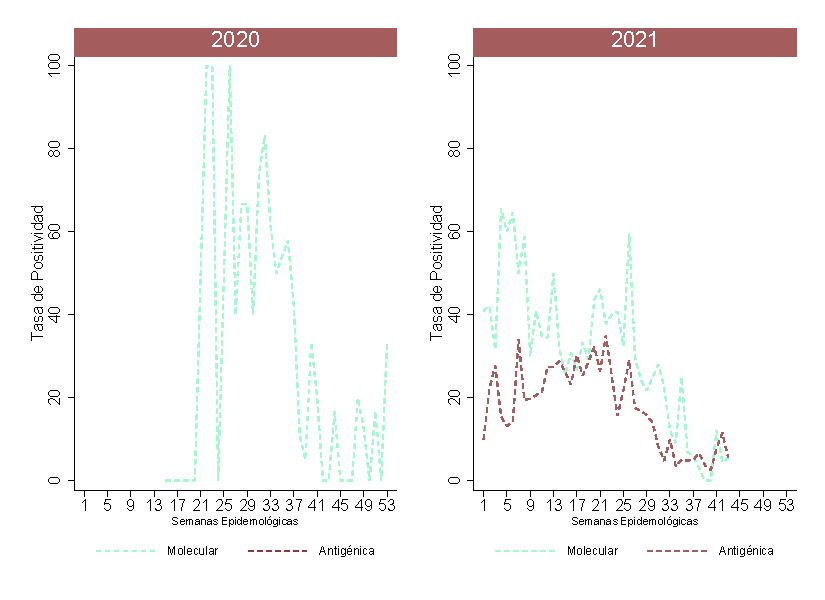
\includegraphics[width=0.8\linewidth, trim={0cm .5cm 0cm 0.2cm},clip]{../figuras/positividad_20_21_12.pdf}
	\end{center}
	{\tiny Fuente de datos: SISCOVID, NOTICOVID.}
\end{frame}

\begin{frame}
	\frametitle{Exceso de Defunciones por Todas las Causas, Provincia Quispicanchi}
	\vspace{-.5cm}
	\begin{center}
		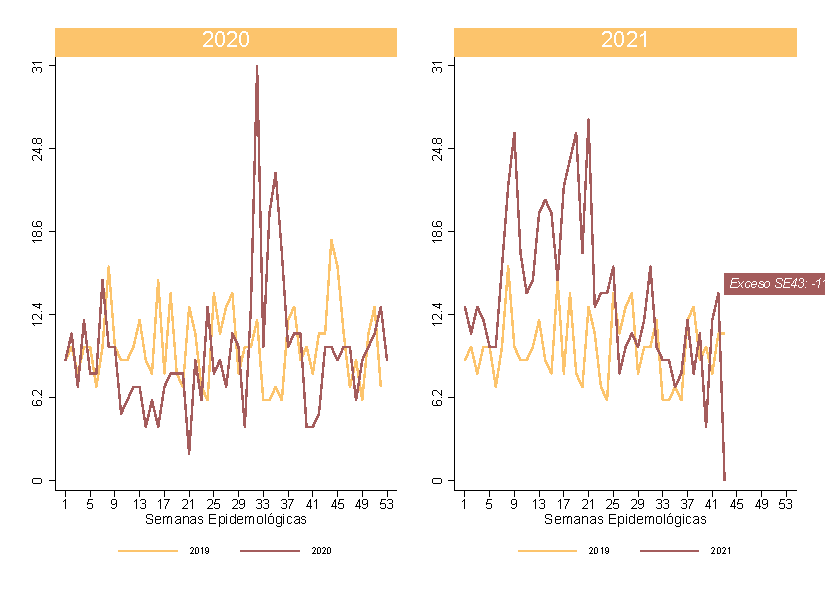
\includegraphics[width=0.8\linewidth, trim={0cm .5cm 0cm 0.2cm},clip]{../figuras/exceso_12.pdf}
	\end{center}
	{\tiny Fuente de datos: SINADEF.}
	
	\hyperlink{indicadores_provinciales}{\beamergotobutton{regresar}}
\end{frame}

\subsection{Urubamba}

\begin{frame}[label=Urubamba]
	\frametitle{\large Incidencia y Mortalidad, Provincia Urubamba}
	\vspace{-.5cm}
	\begin{center}
		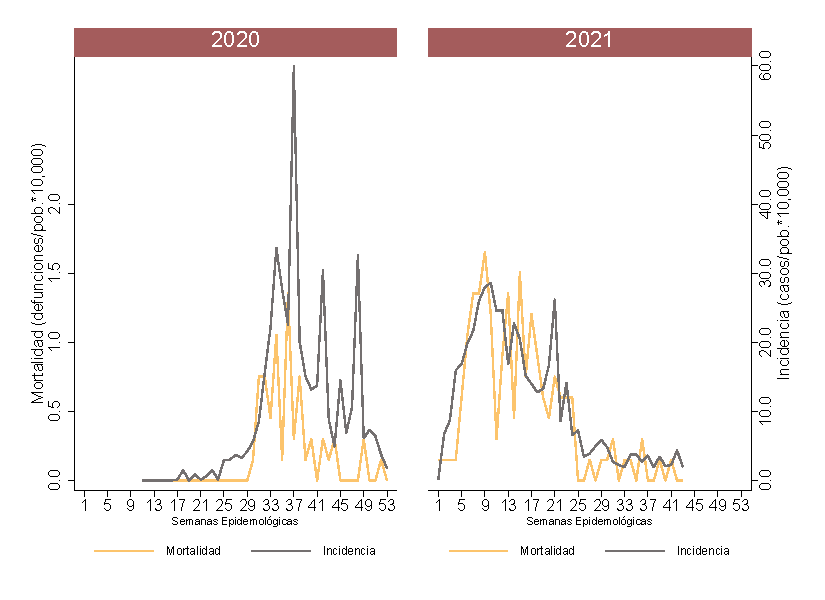
\includegraphics[width=0.8\linewidth, trim={0cm .5cm 0cm 0.2cm},clip]{../figuras/incidencia_mortalidad_20_21_13.pdf}
	\end{center}
	{\tiny Fuente de datos: SISCOVID, NOTICOVID, SINADEF.}
\end{frame}

\begin{frame}
	\frametitle{Tasa de Positividad, Provincia Urubamba}
	\vspace{-.5cm}
	\begin{center}
		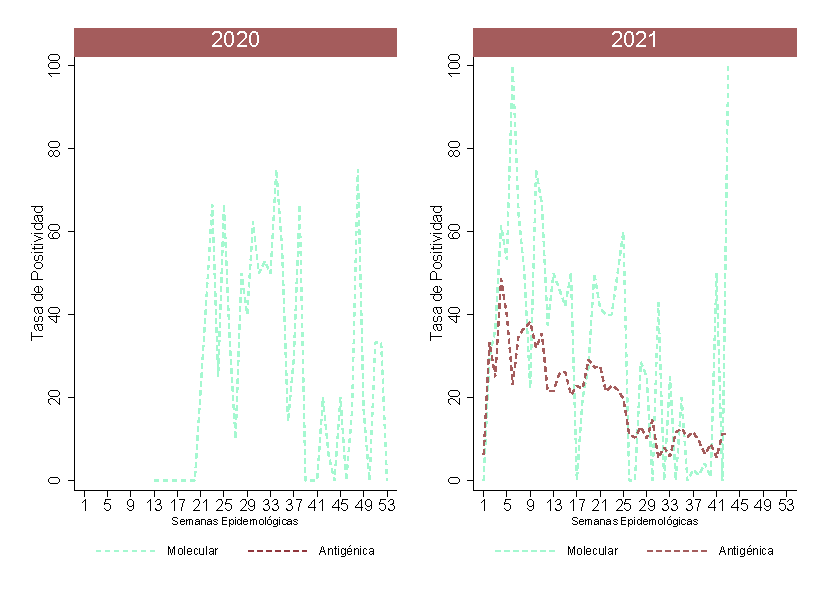
\includegraphics[width=0.8\linewidth, trim={0cm .5cm 0cm 0.2cm},clip]{../figuras/positividad_20_21_13.pdf}
	\end{center}
	{\tiny Fuente de datos: SISCOVID, NOTICOVID.}
\end{frame}

\begin{frame}
	\frametitle{Exceso de Defunciones por Todas las Causas, Provincia Urubamba}
	\vspace{-.5cm}
	\begin{center}
		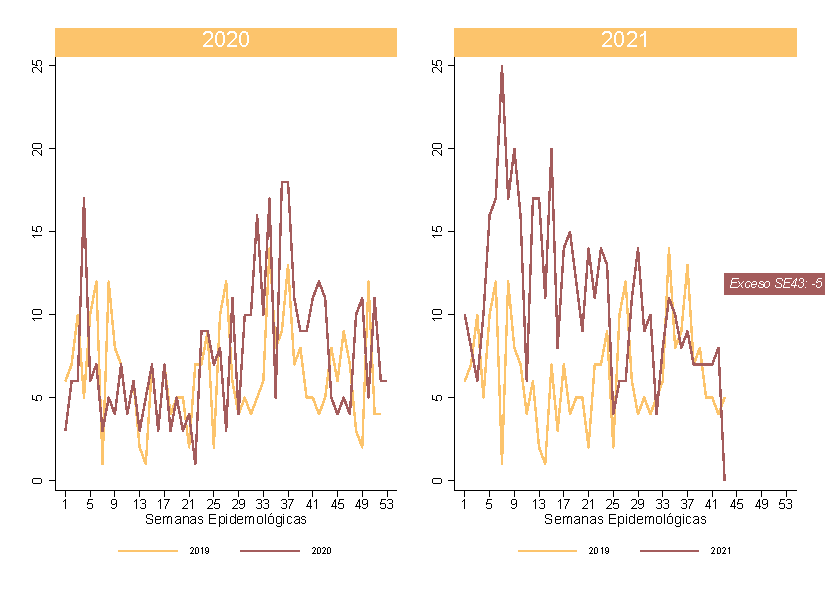
\includegraphics[width=0.8\linewidth, trim={0cm .5cm 0cm 0.2cm},clip]{../figuras/exceso_13.pdf}
	\end{center}
	{\tiny Fuente de datos: SINADEF.} \hyperlink{indice}{\beamergotobutton{Índice}} 
	
	\hyperlink{indicadores_provinciales}{\beamergotobutton{regresar}}
\end{frame}

\subsection{Mapas Variantes}
	\begin{frame}[label=mapa_provincia_cusco]
	\frametitle{Cantidad de Casos Variantes en la Provincia Cusco, 2021}
	\begin{center}
		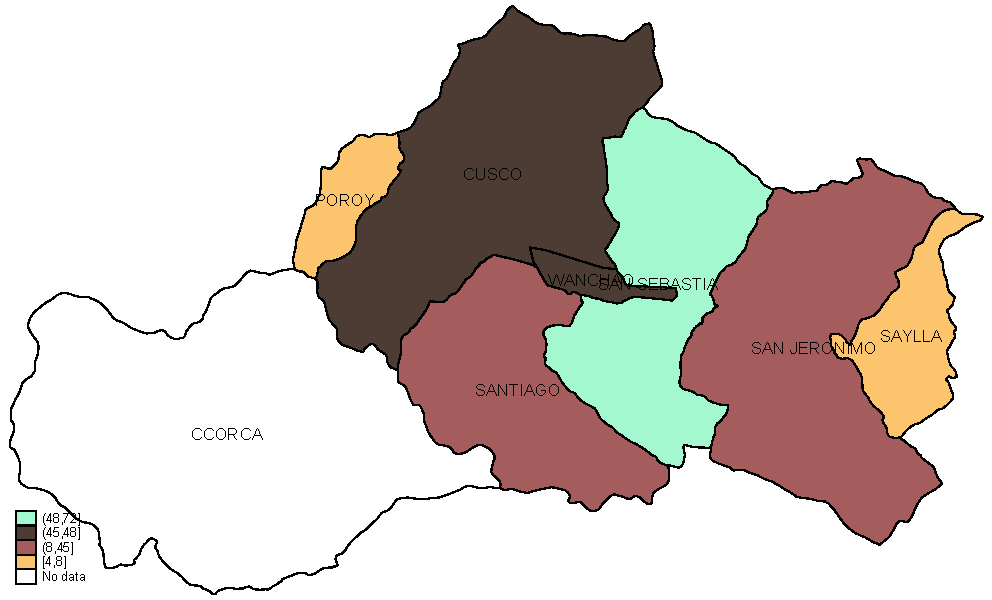
\includegraphics[width=0.65\linewidth]{../figuras/variantes_distrital_cusco.pdf}
	\end{center}
	{\tiny Fuente de datos: NETLAB Cusco, UNSAAC, UPCH.}
	
	\hyperlink{mapa_variantes}{\beamergotobutton{regresar}}
	\end{frame}

	\begin{frame}[label=mapa_distrital]
	\frametitle{Cantidad de Casos Variantes en los Distritos de la Región Cusco, 2021}
	\begin{center}
		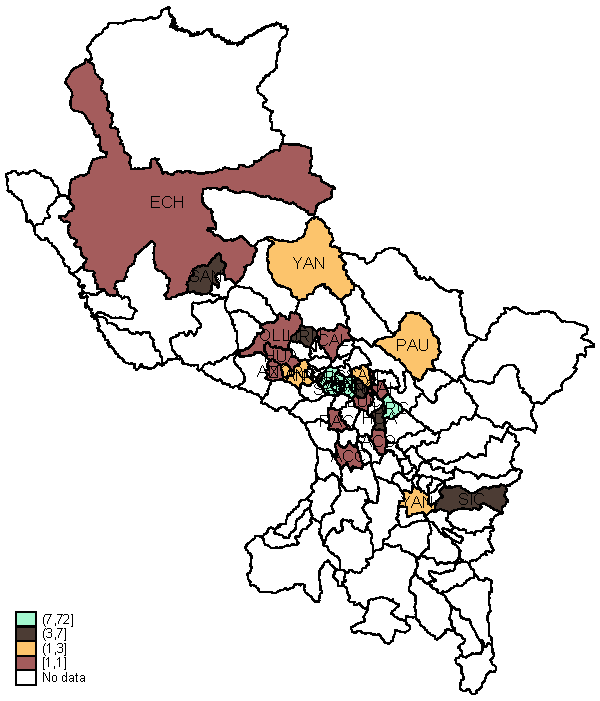
\includegraphics[width=0.55\linewidth]{../figuras/variantes_distrital.pdf}
	\end{center}
	{\tiny Fuente de datos: NETLAB Cusco, UNSAAC, UPCH.}
	
	\hyperlink{mapa_variantes}{\beamergotobutton{regresar}}
	\end{frame}

	\begin{frame}[label=mapa_lambda]
		\frametitle{Cantidad de Casos Variantes \textbf{Lambda} por Provincias, 2021}
		\begin{center}
			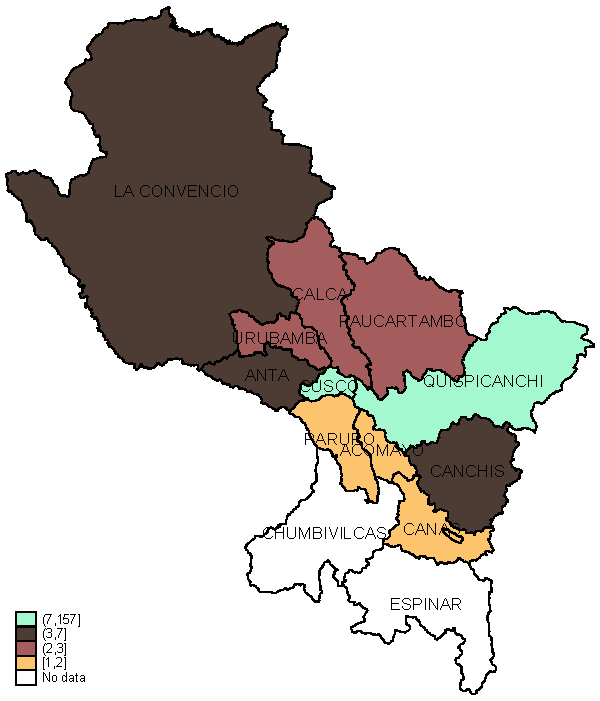
\includegraphics[width=0.55\linewidth]{../figuras/variantes_provincial_lambda.pdf}
		\end{center}
		{\tiny Fuente de datos: NETLAB Cusco, UNSAAC, UPCH.}
		
		\hyperlink{mapa_variantes}{\beamergotobutton{regresar}}
	\end{frame}

	\begin{frame}[label=mapa_gamma]
		\frametitle{Cantidad de Casos  Variante \textbf{Gamma} por Provincias, 2021}
		\begin{center}
			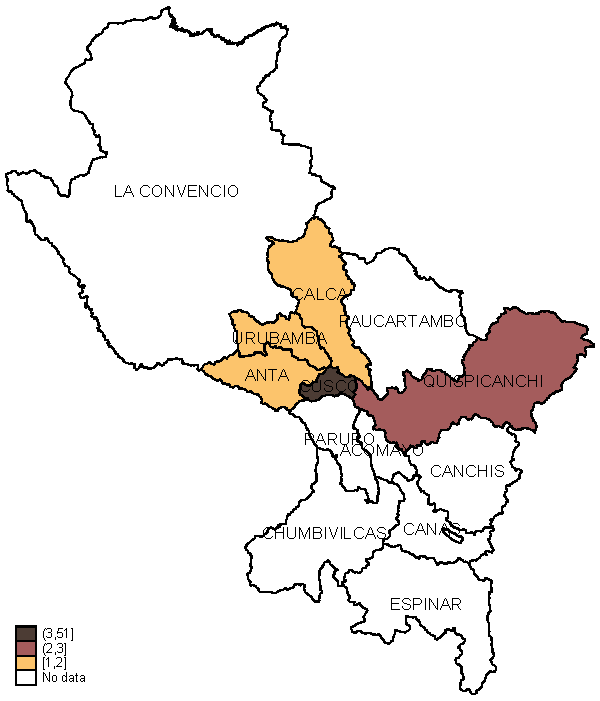
\includegraphics[width=0.55\linewidth]{../figuras/variantes_provincial_gamma.pdf}
		\end{center}
		{\tiny Fuente de datos: NETLAB Cusco, UNSAAC, UPCH.}
		
		\hyperlink{mapa_variantes}{\beamergotobutton{regresar}}
	\end{frame}
	
	\begin{frame}[label=mapa_delta]
		\frametitle{Cantidad de Casos  Variante \textbf{Delta} por Provincias, 2021}
		\begin{center}
			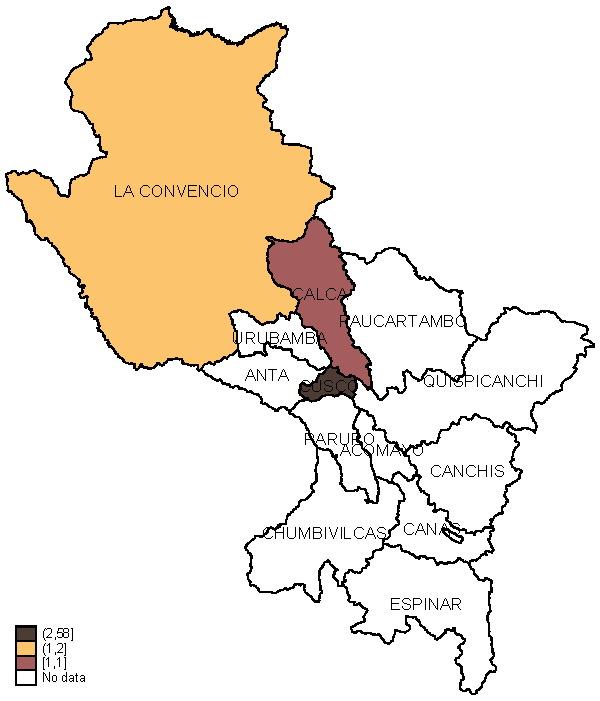
\includegraphics[width=0.55\linewidth]{../figuras/variantes_provincial_delta.pdf}
		\end{center}
		{\tiny Fuente de datos: NETLAB Cusco, UNSAAC, UPCH.}
		
		\hyperlink{mapa_variantes}{\beamergotobutton{regresar}}
	\end{frame}
%\backupend

\end{document}
